\subsection{Famílias conjugadas}

Em muitos dos exemplos que vimos nas seções anteriores,
a priori e a posteriori pertenciam a uma mesma
``família'' de distribuições.
Por exemplo, no \cref{exemplo:eleicao},
consideramos a priori como sendo uma Beta$(5,5)$.
Após observar que uma Binomial$(30,\theta)$ assume o
valor $20$, nossa posteriori segue a
distribuição Beta$(25,15)$. Assim,
tanto a priori quanto a posteriori pertenciam à
família $\text{Beta}$.

O fato de que a priori e a posteriori pertenciam à
mesma família nos exemplos que consideramos não é
uma coincidência. Pelo contrário, os
modelos estatísticos que apresentam esta propriedade são
convenientes computacionalmente e é
justamente por isso que começamos
nossos estudos por eles.
Para entender o motivo desta facilidade computacional,
lembre-se que:
\begin{align*}
 f(\theta_{0}|x)
 &= \frac{f(\theta_{0})f(x|\theta_{0})}
 {\int{f(\theta)f(x|\theta)d\theta}}
\end{align*}
Em geral, a expressão
$\int{f(\theta)f(x|\theta)d\theta}$
pode ser difícil de calcular.
Nestes casos, será difícil obter
$f(\theta_{0}|x)$ diretamente a partir do
Teorema de Bayes (capítulos futuros, analisarão 
o que pode ser feito nesta situação).
Contudo, vimos que, para alguns modelos estatísticos,
pode ser conveniente escrever
\begin{align*}
 f(\theta_{0}|x) \propto f(\theta_{0})f(x|\theta_{0})
\end{align*}
Note que existe uma única constante $K$, tal que 
$\int{Kf(\theta_{0})f(x|\theta_{0})} = 1$.
Assim, como $\int{f(\theta_{0}|x)d\theta}=1$,
se identificarmos que $f(\theta_{0})f(x|\theta_{0})$
é proporcional a uma distribuição,
$g_{a,b}(\theta_{0})$, então podemos concluir que, $f(\theta_{0}|x) =  g_{a,b}(\theta_{0})$.
Observe que, neste caso, sabemos calcular $\int{f(\theta)f(x|\theta)d\theta}$:
\begin{align*}
 f(\theta_{0}|x) 
 &= \frac{\pi(\theta_{0})f(x|\theta_{0})}
 {\int{f(\theta)f(x|\theta)d\theta}} \\
 g_{a,b}(\theta_{0})
 &= \frac{f(\theta_{0})f(x|\theta_{0})}
 {\int{f(\theta)f(x|\theta)d\theta}}
 & f(\theta_{0}|x) = g_{a,b}(\theta_{0}) \\
 \int{f(\theta)f(x|\theta)d\theta}
 &= \frac{f(\theta_{0})f(x|\theta_{0})}
 {g_{a,b}(\theta_{0})}
\end{align*}
No \cref{exemplo:eleicao}, observamos que
$f(\theta_{0})f(x|\theta_{0})$ era
proporcional a uma distribuição Beta(25,15).
Assim, $\int{f(\theta)f(x|\theta)d\theta}$ é
a constante que, dividida por $f(\theta_{0})f(x|\theta_{0})$,
resulta na distribuição Beta$(25,15)$.

É possível formalizar a propriedade que faz com que
saibamos determinar uma distribuição proporcional a
$f(\theta_{0})f(x|\theta_{0})$.
Para tal, considere a seguinte definição
\begin{definition}
 Considere $\mathcal{P}$ como sendo uma família de 
 funções sobre $\Theta$ não-negativas e integráveis.
 Também, seja $f(x|\theta)$ a densidade condicional de
 $x$ dado $\theta$. Dizemos que 
 $\mathcal{P}$ é conjugada para $f(x|\theta)$ se,
 para todo $x \in \chi$,
 $f(\theta_{0}) \in \mathcal{P} \Rightarrow f(x|\theta_{0})f(\theta_{0}) \in \mathcal{P}$.
\end{definition}
Em palavras, se os dados seguem a
distribuição $f(x|\theta)$,
a sua priori para $\theta$ está em $\mathcal{P}$ e
$\mathcal{P}$ é conjugada para $f(x|\theta)$,
então sua posteriori também estará em $\mathcal{P}$.

\begin{example}
 \label{example:bernoulli_conjugate_1}
 Considere $f(x|\theta) = \theta^{x}(1-\theta)^{1-x}$,
 a densidade da Bernoulli$(\theta)$.
 Defina 
 \begin{align*}
  \mathcal{P} = \{f(\theta_{0}): f(\theta_{0}) 
  =K \cdot \theta_{0}^{a-1}(1-\theta_{0})^{b-1},
  (a,b,K) > 0\}
 \end{align*}
 Note que, para todo $f(\theta_{0}) \in \mathcal{P}$,
 \begin{align*}
  f(\theta_{0})f(x|\theta_{0})
  &= K \cdot \theta_{0}^{a-1}(1-\theta_{0})^{b-1}
  \theta_{0}^{x}(1-\theta_{0})^{1-x} \\
  &= K \cdot \theta_{0}^{a+x-1}(1-\theta_{0})^{b+1-x-1}
  \in \mathcal{P}
 \end{align*}
 Portanto, $\mathcal{P}$ é conjugada para
 $f(x|\theta)$.
\end{example}

Em particular, considere que $\mathcal{P}$ é
um conjunto de funções que sabemos integrar.
Se $\mathcal{P}$ é conjugada para $f(x|\theta)$, então para todo $x$,
$f(\theta_{0})f(x|\theta_{0}) \in \mathcal{P}$.
Portanto, sabemos integrar 
$f(\theta_{0})f(x|\theta_{0}) \in \mathcal{P}$, ou seja,
sabemos calcular $\int{f(\theta)f(x|\theta)d\theta}$. Assim, podemos calcular diretamente a posteriori a
partir da equação
\begin{align*}
 f(\theta_{0}|x)
 &= \frac{f(\theta_{0})f(x|\theta_{0})}
 {\int{f(\theta)f(x|\theta)d\theta}}
\end{align*}

\begin{example}
 \label{example:bernoulli_conjugate_2}
 Considere os $\mathcal{P}$ e $f(x|\theta)$ definidos
 no \cref{example:bernoulli_conjugate_1}.
 Sabemos que
 \begin{align*}
  \int{K\theta^{a-1}(1-\theta)^{b-1}d\theta}
  &= K \cdot \beta(a,b)
 \end{align*}
 Portanto,
 \begin{align*}
  f(\theta_{0}|x)
  &= \frac{f(\theta_{0})f(x|\theta_{0})}
  {\int{f(\theta)f(x|\theta)d\theta}} \\
  &= \frac{K\theta_{0}^{a+x-1}(1-\theta_{0})^{b+1-x-1}}
  {\int{K\theta^{a+x-1}(1-\theta)^{b+1-x-1}d\theta}} \\
  &= \frac{K\theta_{0}^{a+x-1}(1-\theta_{0})^{b+1-x-1}}
  {K \cdot \beta(a+x,b+1-x)} \\
  &= \beta^{-1}(a+x,b+1-x)\theta_{0}^{a+x-1}
  (1-\theta_{0})^{b+1-x-1}
 \end{align*}
\end{example}

Em resumo, se $\mathcal{P}$ é conjugada para
$f(x|\theta)$ e sabemos calcular a integral das
funções em $\mathcal{P}$, então podemos calcular
diretamente a posteriori quando usamos uma
priori em $\mathcal{P}$.
Esta é uma das razões pela qual $\mathcal{P}$ é
computacionalmente conveniente.
Também, lembre-se que a densidade preditiva dos dados é
\begin{align*}
 f(x) &= \int{f(\theta)f(x|\theta)d\theta}
\end{align*}
Saber calcular $\int{f(\theta)f(x|\theta)d\theta}$ é
equivalente a saber determinar a
densidade preditiva dos dados.

\begin{lemma}
 Se, dado $\theta$, $X_{1},\ldots,X_{n}$ são i.i.d.
 com densidade 
 dada por $f(x_{1}|\theta)$ e
 $\mathcal{P}$ é conjugada para $f(x_{1}|\theta)$,
 então $\mathcal{P}$ é conjugada para
 $f(x_{1},\ldots,x_{n}|\theta)$.
\end{lemma}

\begin{proof}
 Provaremos o resultado por indução.
 Por definição, $\mathcal{P}$ é conjugada para
 $f(x_{1}|\theta)$.
 Assuma que $\mathcal{P}$ é conjugada para
 $f(x_{1},\ldots,x_{n-1}|\theta)$.
 Note que
 \begin{align*}
  f(\theta) f(x_{1},\ldots,x_{n}|\theta)
  &=f(\theta)f(x_{1},\ldots,x_{n-1}|\theta)
  f(x_{n}|\theta)
  & \text{independência condicional}
 \end{align*}
 Por hipótese de indução $f^{*}(\theta) = f(\theta)f(x_{1},\ldots,x_{n-1}|\theta) \in \mathcal{P}$.
 Como $X_{1}|\theta$ tem mesma distribuição que
 $X_{n}|\theta$ e $f^{*}(\theta) \in \mathcal{P}$,
 conclua que $f^{*}(\theta)f(x_{n}|\theta) \in \mathcal{P}$.
 Assim, $f(\theta) f(x_{1},\ldots,x_{n}|\theta) \in \mathcal{P}$.
\end{proof}

A seguir, estudaremos algumas famílias conjugadas que
são tradicionalmente utilizadas.
Para cada uma delas, derivaremos a forma da posteriori e
a densidade preditiva dos dados.

\subsubsection{O modelo beta-binomial (Dirichlet-multinomial)}
\label{sec:conjugate_beta_binomial}

\begin{lemma}
 \label{lemma:beta-binomial-1}
 Se $X|\theta \sim \text{Binomial}(n,\theta)$, então
 $\mathcal{P} = \{f(\theta): f(\theta) = K \theta^{a-1}(1-\theta)^{b-1}, (a,b,K) > 0\}$
 é conjugada de $f(x|\theta)$.
 Note que todas as densidades em $\mathcal{P}$ são
 da forma $\text{Beta}(a,b)$.
\end{lemma}

\begin{proof}
 \begin{align*}
  f(\theta)f(x|\theta)
  &= {n \choose x}\theta^{x}(1-\theta)^{n-x}
  K \theta^{a-1}(1-\theta)^{b-1} \\
  &= {n \choose x}K \cdot \theta^{a+x-1}
  (1-\theta)^{b+n-x-1} \in \mathcal{P}
 \end{align*}
\end{proof}

\begin{lemma}
 \label{lemma:beta-binomial-2}
 Se $X|\theta \sim \text{Binomial}(n,\theta)$ e
 $\theta \sim \text{Beta}(a,b)$, então
 $\theta|X=x \sim \text{Beta}(a+x,b+n-x)$.
\end{lemma}

\begin{proof}
 \begin{align*}
  f(\theta_{0}|x)
  &= \frac{f(\theta_{0})f(x|\theta_{0})}
  {\int{f(\theta)f(x|\theta)d\theta}} \\
  &= \frac{\beta(a,b)\theta_{0}^{a-1}(1-\theta_{0})^{b-1}
  {n \choose x}\theta_{0}^{x}(1-\theta_{0})^{n-x}}
  {\int{\beta(a,b)\theta^{a-1}(1-\theta)^{b-1}
  {n \choose x}\theta^{x}(1-\theta)^{n-x}d\theta}} \\
  &= \frac{\theta_{0}^{a+x-1}(1-\theta_{0})^{b+n-x-1}}
  {\int{\theta^{a+x-1}(1-\theta)^{b+n-x-1}d\theta}}	\\
  &= \beta^{-1}(a+x,b+n-x)\theta_{0}^{a+x-1}
  (1-\theta_{0})^{b+n-x-1}
 \end{align*}
\end{proof}

\begin{lemma}
 Se $X|\theta \sim \text{Binomial}(n,\theta)$ e
 $\theta \sim \text{Beta}(a,b)$, então:
 \begin{align*}
  f(x) =\frac{\Gamma(a+b)}{\Gamma(a)\Gamma(b)}
  \cdot {n \choose x} \frac{\Gamma(a+x)\Gamma(b+n-x)}
  {\Gamma(a+b+n)}
 \end{align*}
 dizemos que $f(x)$ é a densidade da 
 distribuição Beta-Binomial$(n,a+x,b+n-x)$.
\end{lemma}

\begin{proof}
 \begin{align*}
  f(x)	&= \int{f(x|\theta)f(\theta)d\theta} \\
  &= \int{{n \choose x}\theta^{x}(1-\theta)^{n-x}\beta^{-1}(a,b)\theta^{a-1}(1-\theta)^{b-1}d\theta} \\
  &= {n \choose x}\beta^{-1}(a,b)
  \int{\theta^{a+x-1}(1-\theta)^{b+n-x-1}d\theta} \\
  &= {n \choose x} \beta^{-1}(a,b) \beta(a+x,b+n-x) \\
  &= \frac{\Gamma(a+b)}{\Gamma(a)\Gamma(b)}
  \cdot {n \choose x}\frac{\Gamma(a+x)\Gamma(b+n-x)}
  {\Gamma(a+b+n)}
 \end{align*}
\end{proof}

\begin{definition}
 \label{def:multinomial}
 Dizemos que $\X \in \{0,1\}^d$ tem
 distribuição multinomial com
 parâmetro $(m,\theta)$, para
 $\theta \in \mathbb{R}^d$ tal que
 $\theta_i \geq 0$ e 
 $\sum_{i=1}^{d}\theta_i = 1$, e
 escrevemos $\X \sim \text{Mult}(m,\theta)$ se
 \begin{align*}
  \P(X_1 = x_1, \ldots X_d = x_d|\theta)
  &= \left(\frac{m!}
  {\prod_{j=1}^d x_i!}\prod_{i=1}^d\theta_i^{x_i}\right)
  \I\left(\sum_{i=1}^d x_i = m\right)
 \end{align*}
\end{definition}

\begin{definition}
 \label{def:dirichlet}
 Dizemos que $\theta$ tem
 distribuição Dirichlet com parâmetro
 $\alpha=(\alpha_1,\ldots,\alpha_d) \in \mathbb{R}^d$, onde
 $\alpha_i \geq 0$, e
 escrevemos 
 $\theta \sim \text{Dirichlet}(\alpha)$ se
 \begin{align*}
  f(\theta)
  &= \beta^{-1}(\alpha)
  \left(\prod_{i=1}^{d}\theta_i^{\alpha_i-1}\right)
  \I\left(\sum_{i=1}^d \theta_i = 1\right)
  & \text{, onde }
  \beta(\alpha) 
  = \frac{\prod_{i=1}^d \Gamma(\alpha_i)}
  {\Gamma\left(\sum_{i=1}^d \alpha_i\right)}
 \end{align*}
\end{definition}

\begin{lemma}
 \label{lemma:dirichlet-multinomial}
 Se $\X|\theta \sim \text{Mult}(m,\theta)$, então
 $\mathcal{P} = \left\{f(\theta): 
 f(\theta) = K\prod_{i=1}^d \theta_i^{\alpha_i-1},
 \alpha \in \mathbb{R}^{d}_{+}\right\}$ é
 conjugada para $f(\x|\theta)$. Ademais,
 se $\theta \sim \text{Dirichlet}(\alpha)$, então
 $\theta|\X \sim \text{Dirichlet}(\alpha + \X)$.
\end{lemma}

\begin{proof}
 \begin{align*}
  f(\theta)f(\x|\theta)
  &= \left(\prod_{i=1}^{d}\theta_i^{\alpha_i-1}\right)
  \I\left(\sum_{i=1}^d \theta_i = 1\right)
  \left( \frac{m!}
  {\prod_{j=1}^d x_i!}\prod_{i=1}^d\theta_i^{x_i}\right)
  \I\left(\sum_{i=1}^d x_i = m\right) \\
  &\propto  \left(\prod_{i=1}^d
  {\theta_i^{\alpha_i + x_i-1}}\right)
  \I\left(\sum_{i=1}^d \theta_i = 1\right)
  \in \mathcal{P}
 \end{align*}
\end{proof}

\subsubsection*{Exercícios}

\begin{exercise}
 Considere que, dado $\theta$, 
 $X_{1},\ldots,X_{n}$ são i.i.d 
 $\text{Binomial}(m,\theta)$.
 Também, $\theta \sim \text{Beta}(a,b)$.
 \begin{enumerate}[label=(\alph*)]
  \item Ache a posteriori para $\theta$ após 
  observar $X_{1},\ldots,X_{n}$.
  \item Ache a densidade preditiva para
  $X_{1},\ldots,X_{n}$.
  \item Derive $\lim_{n \rightarrow \infty}\E[\theta|X_{1},\ldots,X_{n}]$. 
  \item Derive $\lim_{n \rightarrow \infty}\V[\theta|X_{1},\ldots,X_{n}]$.
  \item Interprete, em suas palavras,
  os dois itens anteriores.
  \item Calcule o viés, a variância e o erro quadrático médio do estimador $\E[\theta|X_{1},\ldots,X_{n}]$ e compare esses valores com 
  os obtidos pelo estimador de máxima verossimilhança para $\theta$. Interprete.
\end{enumerate}
\end{exercise}

\solution{\textbf{Solução}:
 \begin{enumerate}[label=(\alph*)]
  \item
  \begin{align}
   \label{eqn:beta_bin_1}
   f(\theta|x_{1},\ldots,x_{n})
   &\propto	f(\theta)f(x_{1},\ldots,x_{n}|\theta)
   & \nonumber \\
   &= f(\theta)\prod_{i=1}^{n}{f(x_{i}|\theta)}
   & \text{i.i.d.} \nonumber \\
   &= \beta^{-1}(a,b)\theta^{a-1}(1-\theta)^{b-1}\prod_{i=1}^{n}{{m \choose x_{i}}\theta^{x_{i}}(1-\theta)^{m-x_{i}}}
   & \nonumber \\
   &= \beta^{-1}(a,b)\theta^{a+n\bar{x}-1}(1-\theta)^{b+nm-n\bar{x}-1}\prod_{i=1}^{n}{{m \choose x_{i}}}	  \end{align}
  Note que o resultado da \cref{eqn:beta_bin_1} é
  proporcional à densidade de uma distribuição beta.
  Em particular, obtemos:
  \begin{align*}
   \theta|X_{1},\ldots,X_{n} 
   \sim \text{Beta}(a+n\bar{X},b+nm-n\bar{X})
  \end{align*}
  \item
  \begin{align*}
   f(x_{1},\ldots,x_{n})
   &= \int_{0}^{1}
   {f(\theta)f(x_{1},\ldots,x_{n}|\theta)d\theta} \\
   &= \int_{0}^{1}{\beta^{-1}(a,b)\theta^{a+n\bar{x}-1}(1-\theta)^{b+nm-n\bar{x}-1}\prod_{i=1}^{n}{{m \choose x_{i}}}d\theta} \\
   &= \beta^{-1}(a,b)\prod_{i=1}^{n}{{m \choose x_{i}}}\int_{0}^{1}{\theta^{a+n\bar{x}-1}(1-\theta)^{b+nm-n\bar{x}-1}d\theta} \\
   &= \beta^{-1}(a,b)\beta(a+n\bar{X},b+nm-n\bar{X})\prod_{i=1}^{n}{{m \choose x_{i}}}
  \end{align*}
  
  \item
  \begin{align*}
   \lim_{n \rightarrow \infty}
   \E[\theta|X_{1},\ldots,X_{n}]
   &= \lim_{n \rightarrow \infty} \frac{a+n\bar{X}}
   {a+n\bar{X}+b+nm-n\bar{X}} \\
   &= \lim_{n \rightarrow \infty} \frac{a+n\bar{X}}
   {a+b+nm} \\
   &= \lim_{n \rightarrow \infty}
   \frac{\frac{a}{n}+\bar{X}}{\frac{a+b}{n}+m} \\
   &= m^{-1}\bar{X}
  \end{align*}
  
  \item
  \begin{align*}
   \lim_{n \rightarrow \infty}
   \V[\theta|X_{1},\ldots,X_{n}]
   &= \lim_{n \rightarrow \infty} \frac{(a+n\bar{X})(b+nm-n\bar{X})}{(a+n\bar{X}+b+nm-n\bar{X})^{2}(a+n\bar{X}+b+nm-n\bar{X}+1)} \\
   &= \lim_{n \rightarrow \infty} \frac{n^{2}(\frac{a}{n}+\bar{X})(\frac{b}{n}+(m-\bar{X}))}{n^{3}(\frac{a+b}{n}+m)^{2}(\frac{a+b+1}{n}+m)} = 0
  \end{align*}
 \end{enumerate}
}{}

\begin{exercise}
 Se $\X|\theta \sim \text{Mult}(m,\theta)$ e
 $\theta \sim \text{Dirichlet}(\alpha)$,
 determine $f(\x)$.
\end{exercise}

\subsubsection{O modelo normal-normal}
\label{sec:conj-norm}

O modelo normal é um dos mais usados em Estatística.
Lembre-se que se $X \sim N(\mu,\sigma^{2})$, então:
\begin{align*}
 f(x|\mu,\sigma^{2})
 &= \frac{1}{\sqrt{2\pi}\sigma}
 \exp\left(-\frac{(x-\mu)^{2}}{2\sigma^{2}}\right)
\end{align*}
Para nossa conveniência, usaremos uma 
parametrização do modelo normal diferente da usual.
Definimos $\tau^{2} = \sigma^{-2}$.
Assim, quanto maior o valor de $\tau^{2}$,
menor o valor de $\sigma^{2}$.
Dada esta propriedade, é comum chamarmos
$\tau^{2}$ de \textbf{precisão} da distribuição.
Realizando a substituição adequada, obtemos:
\begin{align*}
 f(x|\mu,\tau^{2})
 &= \frac{\tau}{\sqrt{2\pi}}
 \exp\left(-\frac{\tau^{2}(x-\mu)^{2}}{2}\right)
\end{align*}

A princípio, a distribuição normal pode ter
dois parâmetros, $\mu$ e $\tau^{2}$.
Contudo, como uma simplificação inicial,
consideraremos que $\tau^{2}$ é conhecido e
$\mu$ é desconhecido.
Como candidato para uma família conjugada neste caso, considere,
\begin{align*}
 \mathcal{P} 
 =\left\{f: \mathbb{R} \rightarrow \mathbb{R}^{+}:
 f(\mu) = K \cdot \exp\left(-\frac{\tau_{0}^{2}(\mu-\mu_{0})^{2}}{2}\right) \right\}
\end{align*}
Em outras palavras, $\mathcal{P}$ é o
conjunto de funções proporcionais à densidade de
uma distribuição normal.
Podemos mostrar que $\mathcal{P}$ é
conjugada para a família normal.

\begin{lemma}
 \label{lemma:conjugate_normal_mean}
 Se $\tau^{2}$ é conhecido e
 $X|\mu \sim \text{N}(\mu,\tau^{2})$,
 então
 \begin{align*}
  \mathcal{P} 
  =\left\{f: \mathbb{R} \rightarrow \mathbb{R}^{+}:
  f(\mu) = K \cdot \exp\left(-\frac{\tau_{0}^{2}(\mu-\mu_{0})^{2}}{2}\right) \right\}
 \end{align*}
 é conjugada de $f(x|\mu)$.
 Note que todas as densidades em $\mathcal{P}$ são
 da forma $\text{N}(\mu_{0},\tau_{0}^{2})$.
 Também, se $\mu \sim N(\mu_{0},\tau_{0}^{2})$, então
 \begin{align*}
  \mu|X \sim N\left(\frac{\tau_{0}^{2}\mu_{0}+\tau^{2}x}
  {\tau_{0}^{2}+\tau^{2}},\tau_{0}^{2}+\tau^{2}\right)
 \end{align*}
\end{lemma}

\begin{proof}
 \begin{align}
  \label{eqn:conjugate_normal_1}
  f(\mu) \cdot f(x|\mu)
  &= K \cdot \exp\left(-\frac{\tau_{0}^{2}(\mu-\mu_{0})^{2}}{2}\right)
  \cdot \frac{\tau}{\sqrt{2\pi}} \cdot \exp\left(-\frac{\tau^{2}(x-\mu)^{2}}{2}\right) \nonumber \\
  &\propto \exp\left(-\frac{\tau_{0}^{2}(\mu-\mu_{0})^{2}}{2}\right) \cdot \exp\left(-\frac{\tau^{2}(x-\mu)^{2}}{2}\right)	\nonumber \\
  &= \exp\left(-\frac{\tau_{0}^{2}\mu^{2}-2\tau_{0}^{2}\mu\mu_{0}+\tau^{2}\mu^{2}-2\tau^{2}\mu x}{2}\right) \cdot \exp\left(-\frac{\tau_{0}^{2}\mu_{0}^{2}+\tau^{2}x^{2}}{2}\right) \nonumber \\
  &\propto \exp\left(-\frac{\tau_{0}^{2}\mu^{2}-2\tau_{0}^{2}\mu\mu_{0}+\tau^{2}\mu^{2}-2\tau^{2}\mu x}{2}\right) \nonumber \\
  &= \exp\left(-\frac{(\tau_{0}^{2}+\tau^{2})\mu^{2}-(2\tau_{0}^{2}\mu_{0}+2\tau^{2}x)\mu}{2}\right)
 \end{align}
 Desejamos transformar a expressão da
 \cref{eqn:conjugate_normal_1} em um quadrado perfeito.
 Para tal, observe que:
 \begin{align}
  \label{eqn:conjugate_normal_2}
  \exp\left(-\frac{(a\mu-b)^{2}}{2}\right)
  &= \exp\left(-\frac{a^{2}\mu^{2}-2ab\mu+b^{2}}{2}\right)
 \end{align}

 Para que exista a chance da 
 \cref{eqn:conjugate_normal_1} ser colocada na
 forma da \cref{eqn:conjugate_normal_2},
 é necessário que os coeficientes de $\mu$ sejam
 equivalentes. Assim,
 \begin{align*}
  \begin{cases}
   a^{2} &= \tau_{0}^{2}+\tau^{2} \\
   2ab &= 2\tau_{0}^{2}\mu_{0}+2\tau^{2}x
  \end{cases}
 \end{align*}
 e obtemos
 \begin{align}
  \label{eqn:conjugate_normal_3}
  \begin{cases}
   a &= \sqrt{\tau_{0}^{2}+\tau^{2}} \\
   b &= \frac{\tau_{0}^{2}\mu_{0}+\tau^{2}x}
   {\sqrt{\tau_{0}^{2}+\tau^{2}}}
  \end{cases}
 \end{align}

 Realizando esta substituição na
 \cref{eqn:conjugate_normal_1}, obtemos:
 \begin{align*}
  f(\mu) \cdot f(x|\mu)
  &\propto \exp\left(-\frac{a^{2}\mu^{2}
  -2ab\mu}{2}\right) \\
  &\propto \exp\left(-\frac{a^{2}\mu^{2}
  -2ab\mu+b^{2}}{2}\right)
  & \exp(b^{2}/2) \text{ é constante} \\
  &= \exp\left(-\frac{(a\mu-b)^{2}}{2}\right)
  & \cref{eqn:conjugate_normal_2} \\
  &= \exp\left(-\frac{a^{2}
  \left(\mu-\frac{b}{a}\right)^{2}}{2}\right)
  \in \mathcal{P}
 \end{align*}
 Também observe que $f(\mu) \cdot f(x|\mu)$ é
 proporcional à densidade de uma normal com
 $\mu=\frac{b}{a}$ e $\tau^{2}=a^{2}$.
 Substituindo os valores obtidos na 
 \cref{eqn:conjugate_normal_3} temos que
 \begin{align*}
  \mu|X \sim N\left(\frac{\tau_{0}^{2}\mu_{0}+\tau^{2}x}
  {\tau_{0}^{2}+\tau^{2}},\tau_{0}^{2}+\tau^{2}\right)
 \end{align*}
\end{proof}

Os parâmetros da posteriori no
\cref{lemma:conjugate_normal_mean} ilustram como
a posteriori combina a priori e o dado.
A precisão da posteriori é $\tau_{0}^{2}+\tau^{2}$,
ou seja, a soma das precisões da priori e do dado.
Também, a média da posteriori pode ser reescrita da seguinte forma:
\begin{align*}
 \E[\mu|x]	&= \frac{\tau_{0}^{2}\mu_{0}+\tau^{2}x}
 {\tau_{0}^{2}+\tau^{2}} \\
 &= \mu_{0} \cdot \frac{\tau_{0}^{2}}
 {\tau_{0}^{2}+\tau^{2}}
 +x \cdot \frac{\tau^{2}}{\tau_{0}^{2}+\tau^{2}} \\
 &= \mu_{0} \cdot \frac{\tau_{0}^{2}}
 {\tau_{0}^{2}+\tau^{2}} 
 +x \cdot \left(1-\frac{\tau_{0}^{2}}
 {\tau_{0}^{2}+\tau^{2}}\right)
\end{align*}
Assim, a média da posteriori pode ser escrita como
uma média ponderada (por suas respectivas precisões)
da priori e do dado.

\begin{example} 
\label{ex:altura}
 Considere que desejamos saber  $\mu$, a altura média de um adulto brasileiro.
 Para tanto, vamos assumir que
$\mu \sim N(165,1/100)$.
Medimos então $X$, a altura de um brasileiro selecionado ao acaso.
Se $X|\mu \sim N(\mu,1/25)$ e observamos um indivíduo com $1,8m$ (i.e., $x=180$), então
$\mu|x   \sim N(177,0.05)$. A Figura \ref{fig:normal_normal} mostra a distribuição a priori e a distribuição a posteriori. Note que a posteriori tem a maior parte de sua massa para valores de $\mu$ mais próximos do dado observado. 

\begin{knitrout}
\definecolor{shadecolor}{rgb}{0.969, 0.969, 0.969}\color{fgcolor}\begin{kframe}
\begin{alltt}
\hlkwd{library}\hlstd{(ggplot2)}
\hlstd{grid_mu} \hlkwb{<-} \hlkwd{seq}\hlstd{(}\hlnum{100}\hlstd{,}\hlnum{200}\hlstd{,}\hlkwc{length.out} \hlstd{=} \hlnum{1000}\hlstd{)}

\hlcom{# priori para mu (altura média de um brasileiro)}
\hlstd{mu0} \hlkwb{<-} \hlnum{165}
\hlstd{sigma0} \hlkwb{<-} \hlnum{10}
\hlstd{tau0_2} \hlkwb{<-} \hlnum{1}\hlopt{/}\hlstd{(sigma0)}\hlopt{^}\hlnum{2}
\hlstd{data_plot} \hlkwb{<-} \hlkwd{data.frame}\hlstd{(}\hlkwc{mu}\hlstd{=grid_mu,}
                       \hlkwc{density}\hlstd{=}\hlkwd{dnorm}\hlstd{(grid_mu,mu0,sigma0),}
                       \hlkwc{distribution}\hlstd{=}\hlstr{"Priori"}\hlstd{)}

\hlcom{# dados (altura medida de um indivíduo - normal com média conhecida)}
\hlstd{x} \hlkwb{<-} \hlnum{180}
\hlstd{sigma} \hlkwb{<-} \hlnum{5}
\hlstd{tau_2} \hlkwb{<-} \hlnum{1}\hlopt{/}\hlstd{(sigma)}\hlopt{^}\hlnum{2}

\hlcom{# posteriori}
\hlstd{tau_linha_2} \hlkwb{<-} \hlstd{tau0_2} \hlopt{+} \hlstd{tau_2}
\hlstd{mu_linha} \hlkwb{<-} \hlstd{tau0_2}\hlopt{/}\hlstd{tau_linha_2}\hlopt{*}\hlstd{mu0}\hlopt{+}
 \hlstd{tau_2}\hlopt{/}\hlstd{tau_linha_2}\hlopt{*}\hlstd{x}

\hlstd{data_plot} \hlkwb{<-} \hlkwd{rbind}\hlstd{(data_plot,}
                  \hlkwd{data.frame}\hlstd{(}\hlkwc{mu}\hlstd{=grid_mu,}
                             \hlkwc{density}\hlstd{=}\hlkwd{dnorm}\hlstd{(grid_mu,mu_linha,}\hlnum{1}\hlopt{/}\hlkwd{sqrt}\hlstd{(tau_linha_2)),}
                                           \hlkwc{distribution}\hlstd{=}\hlstr{"Posteriori"}\hlstd{))}

\hlkwd{ggplot}\hlstd{(data_plot)}\hlopt{+}
 \hlkwd{geom_line}\hlstd{(}\hlkwd{aes}\hlstd{(}\hlkwc{x}\hlstd{=mu,}\hlkwc{y}\hlstd{=density,}\hlkwc{color}\hlstd{=distribution),}\hlkwc{size}\hlstd{=}\hlnum{1.2}\hlstd{)}\hlopt{+}
 \hlkwd{theme_minimal}\hlstd{(}\hlkwc{base_size} \hlstd{=} \hlnum{14}\hlstd{)}\hlopt{+}\hlkwd{xlab}\hlstd{(}\hlkwd{expression}\hlstd{(mu))}\hlopt{+}\hlkwd{ylab}\hlstd{(}\hlstr{"Densidade"}\hlstd{)}\hlopt{+}
 \hlkwd{theme}\hlstd{(}\hlkwc{legend.title}\hlstd{=}\hlkwd{element_blank}\hlstd{())}
\end{alltt}


{\ttfamily\noindent\color{warningcolor}{\#\# Warning: Using `size` aesthetic for lines was deprecated in ggplot2 3.4.0.\\\#\# i Please use `linewidth` instead.\\\#\# This warning is displayed once every 8 hours.\\\#\# Call `lifecycle::last\_lifecycle\_warnings()` to see where this warning was\\\#\# generated.}}\end{kframe}\begin{figure}[t]

{\centering 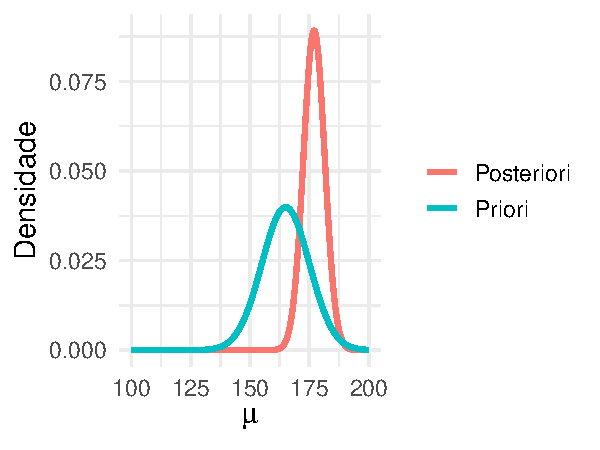
\includegraphics[width=\maxwidth]{./figures/normal_normal-1} 

}

\caption[Distribuições a priori e a posteriori (depois de observamos um indivíduo com 1,8m) para a altura média de um brasileiro]{Distribuições a priori e a posteriori (depois de observamos um indivíduo com 1,8m) para a altura média de um brasileiro}\label{fig:normal_normal}
\end{figure}

\end{knitrout}

\end{example}

A seguir, consideraremos o caso em que
$\mu$ é conhecido e $\tau^{2}$ é desconhecido.
\begin{lemma}
 Se $\mu$ é conhecido e
 $X|\tau^{2} \sim \text{N}(\mu,\tau^{2})$, então
 \begin{align*}
  \mathcal{P} = \left\{f: \mathbb{R} \rightarrow \mathbb{R}^{+}: f(\tau^{2}) = K \cdot \left(\tau^{2}\right)^{\alpha-1} \cdot \exp(-\beta \tau^{2}) \right\}
 \end{align*}
 é conjugada de $f(x|\tau^{2})$.
 Note que todas as densidades em $\mathcal{P}$ são
 da forma $\text{Gamma}(\alpha,\beta)$.
 Também, se $\tau^{2} \sim \text{Gamma}(\alpha,\beta)$,
 então
 \begin{align*}
  \tau^{2}|X \sim \text{Gamma}\left(\alpha+\frac{1}{2},
  \beta+\frac{(X-\mu)^{2}}{2}\right)
 \end{align*}
\end{lemma}

\begin{proof}
 \begin{align*}
  f(\tau^{2}) \cdot f(x|\mu)
  &= K \cdot \left(\tau^{2}\right)^{\alpha-1} \cdot \exp(-\beta \tau^{2}) \cdot \frac{\tau}{\sqrt{2\pi}} \cdot \exp\left(-\frac{\tau^{2}(x-\mu)^{2}}{2}\right)
  \nonumber \\
  &\propto \left(\tau^{2}\right)^{\alpha-1} \cdot \tau \cdot \exp(-\beta \tau^{2}) \cdot \exp\left(-\frac{\tau^{2}(x-\mu)^{2}}{2}\right) \\
  &= \left(\tau^{2}\right)^{\alpha+\frac{1}{2}-1} \cdot \exp\left(-\left(\beta+\frac{(x-\mu)^{2}}{2}\right)\tau^{2}\right) \in \mathcal{P}
 \end{align*}
 Também observe que $f(\tau^{2}) \cdot f(x|\tau^{2})$ é
 proporcional à densidade de uma Gamma com parâmetros
 $\alpha+\frac{1}{2}$ e
 $\left(\beta+\frac{(x-\mu)^{2}}{2}\right)$. Portanto,
 \begin{align*}
  \tau^{2}|X \sim \text{Gamma}\left(\alpha+\frac{1}{2},
  \beta+\frac{(x-\mu)^{2}}{2}\right).
 \end{align*}
\end{proof}

Finalmente, prosseguimos ao caso em que
tanto $\mu$ quanto $\tau^{2}$ são desconhecidos
\begin{lemma}
 \label{lemma:conjugate_normal_mean_precision}
 Se $X|\mu,\tau^{2} \sim \text{N}(\mu,\tau^{2})$,
 então
 \begin{align*}
  \mathcal{P} = \left\{f: \mathbb{R} \rightarrow \mathbb{R}^{+}: f(\mu) = K \cdot (\tau^{2})^{\alpha-1}\exp(-\beta \tau^{2})\exp\left(-\frac{\lambda\tau^{2}(\mu-\mu_{0})^{2}}{2}\right)\right\}
 \end{align*}
 é conjugada de $f(x|\mu,\tau^{2})$.
 As densidades em $\mathcal{P}$ pertencem à
 família bivariada Normal-Gamma com parâmetros
 $(\mu_{0},\lambda,\alpha,\beta)$. Note que se 
 $(\mu,\tau^{2})$ tem distribuição Normal-Gamma,
 então $\mu$ e $\tau^{2}$ não são independentes.
 De fato, se $(\mu,\tau^{2}) \sim \text{Normal-Gamma}(\mu_{0},\lambda,\alpha,\beta)$, então temos:
 \begin{align*}
  \tau^{2} \sim \text{Gamma}(\alpha, \beta) \\
  \mu|\tau^{2} \sim \text{Normal}(\mu_{0},\lambda \tau^{2})
 \end{align*}
 Também, se $(\mu,\tau^{2}) \sim \text{Normal-Gamma}(\alpha,\beta,\mu_{0},\lambda)$, então
 \begin{align*}
  (\mu,\tau^{2})|X \sim \text{Normal-Gamma}\left(\frac{(\lambda\mu_{0}+X)}{\lambda+1}, \lambda+1, \alpha+\frac{1}{2}, \beta + \frac{\lambda(\mu_{0}-X)^{2}}{2(\lambda+1)} \right)
 \end{align*}
\end{lemma}

\begin{proof}
 Note que, nos passos a seguir, tanto
 $\mu$ quanto $\tau^{2}$ são desconhecidos.
 Assim, expressões que dependam de
 quaisquer destes parâmetros não são constantes.
 \begin{align}
  \label{eqn:conjugate_normal_mean_variance_1}
  f(\mu,\tau^{2}|x)
  &\propto f(\mu,\tau^{2})f(x|\mu,\tau^{2})	\nonumber \\
  &= K \cdot (\tau^{2})^{\alpha-1}\exp(-\beta \tau^{2})\exp\left(-\frac{\lambda\tau^{2}(\mu-\mu_{0})^{2}}{2}\right) \cdot \frac{\tau}{\sqrt{2\pi}}\exp\left(-\frac{\tau^{2}(x-\mu)^{2}}{2}\right) \nonumber \\
  &\propto (\tau^{2})^{\alpha+\frac{1}{2}-1} \cdot \exp(-\beta \tau^{2}) \cdot \exp\left(-\frac{\lambda\tau^{2}(\mu^{2}-2\mu\mu_{0}+\mu_{0}^{2})}{2}\right) \cdot \exp\left(-\frac{\tau^{2}(x^{2}-2x\mu+\mu^{2})}{2}\right)	\nonumber \\
  &= (\tau^{2})^{\alpha+\frac{1}{2}-1} \cdot \exp\left(-\left(\beta + \frac{x^{2}}{2} + \frac{\lambda\mu_{0}^{2}}{2}\right)\tau^{2}\right) \cdot \exp\left(-\frac{\lambda\tau^{2}\mu^{2}-2\lambda\tau^{2}\mu\mu_{0}+\tau^{2}\mu^{2}-2\tau^{2}x\mu}{2}\right) \nonumber \\
  &= (\tau^{2})^{\alpha+\frac{1}{2}-1} \cdot \exp\left(-\left(\beta + \frac{x^{2}}{2} + \frac{\lambda\mu_{0}^{2}}{2}\right)\tau^{2}\right) \cdot \exp\left(-\frac{(\lambda+1)\tau^{2}\mu^{2}-2(\lambda\tau^{2}\mu_{0}+\tau^{2}x)\mu}{2}\right)
 \end{align}
 Similarmente ao caso em que $\tau^{2}$ é conhecido,
 desejamos completar o quadrado em função de
 $\mu$ para obter o formato da distribuição normal.
 Usamos novamente a \cref{eqn:conjugate_normal_2} para
 obter
 \begin{align*}
  \begin{cases}
   a^{2} &= (\lambda+1)\tau^{2} \\
   2ab &= 2(\lambda\tau^{2}\mu_{0}+\tau^{2}x)
  \end{cases}
 \end{align*}
 e obtemos
 \begin{align}
  \label{eqn:conjugate_normal_mean_variance_2}
  \begin{cases}
   a &= \sqrt{\lambda+1} \cdot \tau \\
   b &= \frac{\tau(\lambda\mu_{0}+x)}{\sqrt{\lambda+1}}
  \end{cases}
 \end{align}
 Substituindo a
 \cref{eqn:conjugate_normal_mean_variance_2}
 em \cref{eqn:conjugate_normal_mean_variance_1}, obtemos:
 \begin{align*}
  f(\mu,\tau^{2}|x) &\propto (\tau^{2})^{\alpha+\frac{1}{2}-1} \cdot \exp\left(-\left(\beta + \frac{x^{2}}{2} + \frac{\lambda\mu_{0}^{2}}{2}\right)\tau^{2}\right) \cdot \exp\left(-\frac{a^{2}\mu^{2}-2ab\mu}{2}\right) \\
  &= (\tau^{2})^{\alpha+\frac{1}{2}-1} \cdot \exp\left(-\left(\beta + \frac{x^{2}}{2} + \frac{\lambda\mu_{0}^{2}}{2}\right)\tau^{2}\right) \cdot \exp\left(-\frac{a^{2}\mu^{2}-2ab\mu+b^{2}}{2}\right) \cdot \exp\left(\frac{b^{2}}{2}\right) \\
  &= (\tau^{2})^{\alpha+\frac{1}{2}-1} \cdot \exp\left(-\left(\beta + \frac{x^{2}}{2} + \frac{\lambda\mu_{0}^{2}}{2}\right)\tau^{2} + \frac{b^{2}}{2}\right) \cdot \exp\left(-\frac{a^{2}\left(\mu-\frac{b}{a}\right)^{2}}{2}\right) \\
  &= (\tau^{2})^{\alpha+\frac{1}{2}-1} \cdot \exp\left(-\left(\beta + \frac{x^{2}}{2} + \frac{\lambda\mu_{0}^{2}}{2}\right)\tau^{2} + \frac{\tau^{2} (\lambda\mu_{0}+x)^{2}}{2(\lambda+1)}\right) \cdot \exp\left(-\frac{a^{2}\left(\mu-\frac{b}{a}\right)^{2}}{2}\right) \\
  &= (\tau^{2})^{\alpha+\frac{1}{2}-1} \cdot \exp\left(-\left(\beta + \frac{x^{2}}{2} + \frac{\lambda\mu_{0}^{2}}{2}\right)\tau^{2} + \frac{\tau^{2} (\lambda\mu_{0}+x)^{2}}{2(\lambda+1)}\right) \cdot \exp\left(-\frac{a^{2}\left(\mu-\frac{b}{a}\right)^{2}}{2}\right) \\
  &= (\tau^{2})^{\alpha+\frac{1}{2}-1} \cdot \exp\left(-\left(\beta + \frac{\lambda(\mu_{0}-x)^{2}}{2(\lambda+1)}\right)\tau^{2}\right) \cdot \exp\left(-\frac{a^{2}\left(\mu-\frac{b}{a}\right)^{2}}{2}\right)	\\
  &= (\tau^{2})^{\alpha+\frac{1}{2}-1} \cdot \exp\left(-\left(\beta + \frac{\lambda(\mu_{0}-x)^{2}}{2(\lambda+1)}\right)\tau^{2}\right) \cdot \exp\left(-\frac{(\lambda+1)\tau^{2}\left(\mu-\frac{(\lambda\mu_{0}+x)}{\lambda+1}\right)^{2}}{2}\right) \in \mathcal{P}
 \end{align*}
 Do resultado acima, podemos concluir que
 \begin{align*}
  (\mu,\tau^{2})|X \sim \text{Normal-Gamma}\left(\frac{(\lambda\mu_{0}+X)}{\lambda+1}, \lambda+1, \alpha+\frac{1}{2}, \beta + \frac{\lambda(\mu_{0}-X)^{2}}{2(\lambda+1)} \right)
 \end{align*}
\end{proof}


\begin{example}
 Considere novamente o Exemplo
 \ref{ex:altura}, mas vamos agora assumir 
 que a altura de um brasileiro selecionado ao acaso, 
 $X$, é tal que
 $X|\mu \sim N(\mu,\tau^2)$, 
 com $\tau^2$ desconhecido.
 Agora precisamos fazer a inferência simultaneamente 
 para $\mu$ e $\tau^2$
 Para tanto, vamos assumir que
 $(\mu,\tau^2) \sim \mbox{Normal-Gamma}(1.65,1,6,0.05)$.
 Como $x=1.8$,
 $(\mu,\tau^2)|x \sim 
 \mbox{Normal-Gamma}(1.725, 2, 6.5, 0.055625)$. 
 A Figura \ref{fig:normal_gamma} mostra 
 a distribuição a priori e 
 a distribuição a posteriori 
 para essa observação. 

\begin{knitrout}
\definecolor{shadecolor}{rgb}{0.969, 0.969, 0.969}\color{fgcolor}\begin{kframe}
\begin{alltt}
\hlkwd{library}\hlstd{(ggplot2)}
\hlkwd{library}\hlstd{(patchwork)}

\hlkwd{set.seed}\hlstd{(}\hlnum{0}\hlstd{)}
\hlstd{sigma} \hlkwb{<-} \hlnum{0.075}
\hlstd{mu} \hlkwb{<-} \hlnum{1.70}
\hlcom{# X ~ N(mu, sigma)}
\hlstd{altura} \hlkwb{<-} \hlnum{1.80}

\hlstd{atualiza} \hlkwb{<-} \hlkwa{function}\hlstd{(}\hlkwc{hparam}\hlstd{,} \hlkwc{x}\hlstd{)}
\hlstd{\{}
  \hlkwd{list}\hlstd{(}
    \hlkwc{mu0} \hlstd{= (hparam}\hlopt{$}\hlstd{lambda}\hlopt{*}\hlstd{hparam}\hlopt{$}\hlstd{mu0}\hlopt{+}\hlstd{x)}\hlopt{/}\hlstd{(hparam}\hlopt{$}\hlstd{lambda}\hlopt{+}\hlnum{1}\hlstd{),}
    \hlkwc{lambda} \hlstd{= hparam}\hlopt{$}\hlstd{lambda} \hlopt{+} \hlnum{1}\hlstd{,}
    \hlkwc{alpha} \hlstd{= hparam}\hlopt{$}\hlstd{alpha} \hlopt{+} \hlnum{.5}\hlstd{,}
    \hlkwc{beta} \hlstd{= hparam}\hlopt{$}\hlstd{beta} \hlopt{+}
      \hlstd{(hparam}\hlopt{$}\hlstd{lambda}\hlopt{*}\hlstd{(hparam}\hlopt{$}\hlstd{mu0}\hlopt{-}\hlstd{x)}\hlopt{^}\hlnum{2}\hlstd{)}\hlopt{/}\hlstd{(}\hlnum{2}\hlopt{*}\hlstd{(hparam}\hlopt{$}\hlstd{lambda}\hlopt{+}\hlnum{1}\hlstd{))}
  \hlstd{)}
\hlstd{\}}

\hlstd{hparam_prior} \hlkwb{<-} \hlkwd{list}\hlstd{(}
  \hlkwc{mu0} \hlstd{=} \hlnum{1.65}\hlstd{,}
  \hlkwc{lambda} \hlstd{=} \hlnum{1}\hlstd{,}
  \hlkwc{beta} \hlstd{=} \hlnum{0.05}\hlstd{,}
  \hlkwc{alpha} \hlstd{=} \hlnum{120}\hlopt{*}\hlnum{0.05}
\hlstd{)}

\hlstd{grid_bivariado} \hlkwb{<-} \hlkwd{expand.grid}\hlstd{(}
  \hlkwc{mu} \hlstd{=} \hlkwd{seq}\hlstd{(}\hlnum{1.4}\hlstd{,} \hlnum{1.8}\hlstd{,} \hlkwc{length.out} \hlstd{=} \hlnum{300}\hlstd{),}
  \hlkwc{tau2} \hlstd{=} \hlkwd{seq}\hlstd{(}\hlnum{60}\hlstd{,} \hlnum{200}\hlstd{,} \hlkwc{length.out} \hlstd{=} \hlnum{300}\hlstd{)}
\hlstd{)}

\hlcom{# retorna f(grid_bivariado|hparam)}
\hlstd{densidade} \hlkwb{<-} \hlkwa{function}\hlstd{(}\hlkwc{grid_bivariado}\hlstd{,} \hlkwc{hparam}\hlstd{)}
\hlstd{\{}
  \hlkwd{dgamma}\hlstd{(grid_bivariado}\hlopt{$}\hlstd{tau2,}
         \hlstd{hparam}\hlopt{$}\hlstd{alpha,}
         \hlstd{hparam}\hlopt{$}\hlstd{beta)}\hlopt{*}
    \hlkwd{dnorm}\hlstd{(grid_bivariado}\hlopt{$}\hlstd{mu,}
          \hlstd{hparam}\hlopt{$}\hlstd{mu0,}
          \hlkwd{sqrt}\hlstd{(}\hlnum{1}\hlopt{/}\hlstd{(hparam}\hlopt{$}\hlstd{lambda}\hlopt{*}\hlstd{grid_bivariado}\hlopt{$}\hlstd{tau2)))}
\hlstd{\}}

\hlstd{plot_densidade} \hlkwb{<-} \hlkwa{function}\hlstd{(}\hlkwc{grid_bivariado}\hlstd{,} \hlkwc{hparam}\hlstd{)}
\hlstd{\{}
  \hlstd{dados_plot} \hlkwb{<-} \hlkwd{data.frame}\hlstd{(}
    \hlkwc{mu} \hlstd{= grid_bivariado}\hlopt{$}\hlstd{mu,}
    \hlkwc{tau2} \hlstd{= grid_bivariado}\hlopt{$}\hlstd{tau2,}
    \hlkwc{densidade} \hlstd{=} \hlkwd{densidade}\hlstd{(grid_bivariado, hparam)}
  \hlstd{)}

  \hlkwd{ggplot}\hlstd{(dados_plot,}
         \hlkwd{aes}\hlstd{(mu, tau2,} \hlkwc{fill} \hlstd{= densidade))} \hlopt{+}
    \hlkwd{geom_raster}\hlstd{(}\hlkwc{interpolate} \hlstd{=} \hlnum{TRUE}\hlstd{)} \hlopt{+}
    \hlkwd{ggtitle}\hlstd{(}\hlkwd{paste0}\hlstd{(}\hlstr{"Prior"}\hlstd{))} \hlopt{+}
    \hlkwd{coord_cartesian}\hlstd{(}\hlkwc{xlim}\hlstd{=}\hlkwd{range}\hlstd{(grid_bivariado}\hlopt{$}\hlstd{mu),}
                    \hlkwc{ylim}\hlstd{=}\hlkwd{range}\hlstd{(grid_bivariado}\hlopt{$}\hlstd{tau2))} \hlopt{+}
    \hlkwd{scale_fill_gradientn}\hlstd{(}\hlkwc{colours} \hlstd{=} \hlkwd{terrain.colors}\hlstd{(}\hlnum{100}\hlstd{))} \hlopt{+}
    \hlkwd{theme_bw}\hlstd{()} \hlopt{+}
    \hlkwd{theme}\hlstd{(}\hlkwc{axis.text}\hlstd{=}\hlkwd{element_text}\hlstd{(}\hlkwc{size}\hlstd{=}\hlnum{18}\hlstd{),}
          \hlkwc{axis.title}\hlstd{=}\hlkwd{element_text}\hlstd{(}\hlkwc{size}\hlstd{=}\hlnum{20}\hlstd{,}\hlkwc{face}\hlstd{=}\hlstr{"bold"}\hlstd{))} \hlopt{+}
    \hlkwd{xlab}\hlstd{(}\hlkwd{expression}\hlstd{(mu))} \hlopt{+}
    \hlkwd{ylab}\hlstd{(}\hlkwd{expression}\hlstd{(tau}\hlopt{^}\hlnum{2}\hlstd{))}
\hlstd{\}}

\hlstd{aux1} \hlkwb{=} \hlkwd{plot_densidade}\hlstd{(grid_bivariado, hparam_prior)}
\hlstd{aux2} \hlkwb{=} \hlkwd{plot_densidade}\hlstd{(grid_bivariado,}
                      \hlkwd{atualiza}\hlstd{(hparam_prior, altura))}

\hlstd{aux1}
\end{alltt}
\end{kframe}\begin{figure}[t]

{\centering 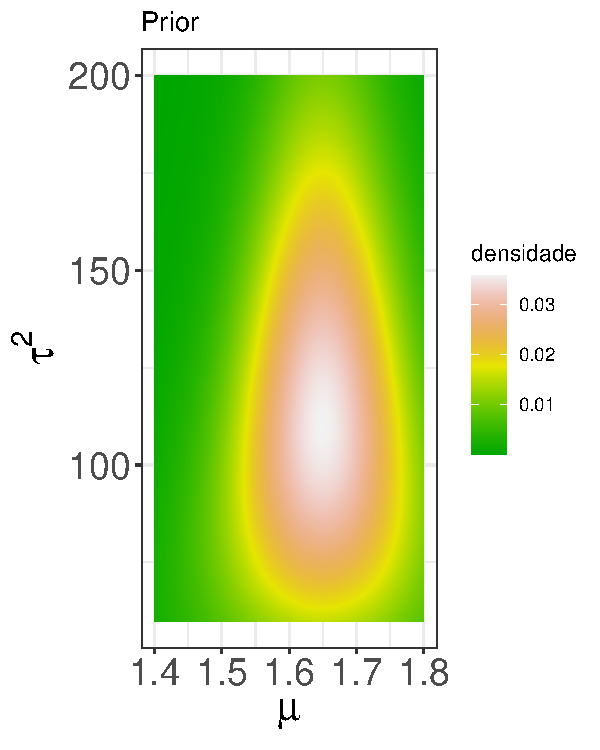
\includegraphics[width=\maxwidth]{figure/normal_gamma-1} 

}

\caption[Distribuições a priori e a posteriori (depois de observamos um indivíduo com 1,8m) para a altura média de um brasileiro]{Distribuições a priori e a posteriori (depois de observamos um indivíduo com 1,8m) para a altura média de um brasileiro}\label{fig:normal_gamma-1}
\end{figure}

\begin{kframe}\begin{alltt}
\hlstd{aux2}
\end{alltt}
\end{kframe}\begin{figure}[t]

{\centering 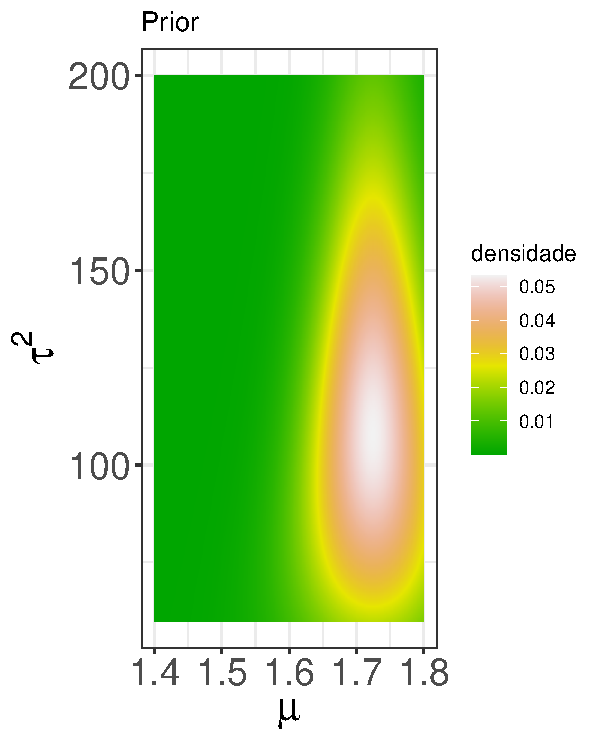
\includegraphics[width=\maxwidth]{figure/normal_gamma-2} 

}

\caption[Distribuições a priori e a posteriori (depois de observamos um indivíduo com 1,8m) para a altura média de um brasileiro]{Distribuições a priori e a posteriori (depois de observamos um indivíduo com 1,8m) para a altura média de um brasileiro}\label{fig:normal_gamma-2}
\end{figure}

\end{knitrout}
\end{example}

\subsubsection*{Exercícios}

\begin{exercise}
 \label{ex:conjugate-normal-normal}
 Considere que, dado $\mu$,
 $X_{1},\ldots,X_{n}$ são i.i.d. e
 $X_{i} \sim N(\mu,\tau^{2})$, com
 $\tau^{2}$ conhecido. Se
 $\mu \sim N(\mu_{0},\tau_{0}^{2})$, então:
 \begin{enumerate}[label=(\alph*)]
  \item Ache a posteriori para
  $\mu|X_{1},\ldots,X_{n}$.
  \item Determine 
  $\lim_{n \rightarrow \infty}\E[\mu|X_{1},\ldots,X_{n}]$.
  \item Determine
  $\lim_{n \rightarrow \infty}\V[\mu|X_{1},\ldots,X_{n}]$.
  \item Interprete em suas próprias palavras os
  resultados obtidos nos itens anteriores.
 \end{enumerate}
\end{exercise}

\solution{\textbf{Solução}:
 \begin{enumerate}[label=(\alph*)]
  \item
  \begin{align*}
   f(\mu) \cdot f(x_{1},\ldots,x_{n}|\mu)
   &= f(\mu)\prod_{i=1}^{n}{f(x_{i}|\mu)} \\
   &\propto \exp\left(-\frac{\tau_{0}^{2}(\mu-\mu_{0})^{2}}{2}\right) \cdot \prod_{i=1}^{n}{\exp\left(-\frac{\tau^{2}(x_{i}-\mu)^{2}}{2}\right)} \\
   &= \exp\left(-\frac{\tau_{0}^{2}\mu^{2}-2\tau_{0}^{2}\mu\mu_{0}+\tau_{0}^{2}\mu_{0}^{2}}{2}\right) \cdot \exp\left(-\frac{n\tau^{2}\mu^{2}-2\tau^{2}\mu \sum_{i=1}^{n}{x_{i}}+ \tau^{2}\sum_{i=1}^{n}{x_{i}^{2}}}{2}\right)	\nonumber \\
   &\propto \exp\left(-\frac{\tau_{0}^{2}\mu^{2}-2\tau_{0}^{2}\mu\mu_{0}+n\tau^{2}\mu^{2}-2n\tau^{2}\mu \bar{x}}{2}\right) \\
   &= \exp\left(-\frac{(\tau_{0}^{2}+n\tau^{2})\mu^{2}-2(\tau_{0}^{2}\mu_{0}+n\tau^{2}\bar{x})\mu}{2}\right)
  \end{align*}
  Realizando uma substituição de acordo com a
  \cref{eqn:conjugate_normal_2}, obtemos
  \begin{align*}
   \begin{cases}
    a^{2} &= \tau_{0}^{2}+n\tau^{2} \\
    2ab &= 2(\tau_{0}^{2}\mu_{0}+n\tau^{2}\bar{x})
   \end{cases}
  \end{align*}
  e
  \begin{align}
   \begin{cases}
    a &= \sqrt{\tau_{0}^{2}+n\tau^{2}} \\
    b &= \frac{\tau_{0}^{2}\mu_{0}+n\tau^{2}\bar{x}}
    {\sqrt{\tau_{0}^{2}+n\tau^{2}}}
   \end{cases}
  \end{align}
  Realizando esta substituição na
  \cref{eqn:conjugate_normal_1}, obtemos:
  \begin{align*}
   f(\mu) \cdot f(x|\mu)
   &\propto \exp\left(-\frac{a^{2}\mu^{2}
   -2ab\mu}{2}\right) \\
   &\propto \exp\left(-\frac{a^{2}\mu^{2}
   -2ab\mu+b^{2}}{2}\right)
   & \exp(b^{2}/2) \text{ é constante} \\
   &= \exp\left(-\frac{(a\mu-b)^{2}}{2}\right)
   & \cref{eqn:conjugate_normal_2} \\
   &= \exp\left(-\frac{a^{2}\left(\mu
   -\frac{b}{a}\right)^{2}}{2}\right) \in \mathcal{P}
  \end{align*}
  Também observe que $f(\mu) \cdot f(x|\mu)$ é
  proporcional à densidade de uma normal com
  $\mu=\frac{b}{a}$ e $\tau^{2}=a^{2}$.
  Substituindo os valores obtidos na   
  \cref{eqn:conjugate_normal_3} temos que
  \begin{align*}
   \mu|X_{1},\ldots,X_{n} \sim
   N\left(\frac{\tau_{0}^{2}\mu_{0}+n\tau^{2}\bar{x}}{\tau_{0}^{2}+n\tau^{2}},\tau_{0}^{2}+n\tau^{2}\right)
  \end{align*}

  \item
  \begin{align*}
   \lim_{n \rightarrow \infty}E[\mu|X_{1},\ldots,X_{n}]	
   &= \lim_{n \rightarrow \infty}
   \frac{\tau_{0}^{2}\mu_{0}+n\tau^{2}\bar{X}}
   {\tau_{0}^{2}+n\tau^{2}} \\
   &= \lim_{n \rightarrow \infty}
   \frac{\tau_{0}^{2}\mu_{0}/n +\tau^{2}\bar{X}}
   {\tau_{0}^{2}/n +\tau^{2}} = \bar{X} \\
  \end{align*}

  \item 
  \begin{align*}
   \lim_{n \rightarrow \infty}
   \V[\mu|X_{1},\ldots,X_{n}]
   &= \lim_{n \rightarrow \infty}
   \frac{1}{\tau_{0}^{2}+n\tau^{2}} = 0
  \end{align*}
 \end{enumerate}
}{}

\begin{exercise}
 Considere que, dado $\tau^{2}$,
 $X_{1},\ldots,X_{n}$ são i.i.d. e
 $X_{i} \sim N(\mu,\tau^{2})$, com
 $\mu$ conhecido. Considere que
 $\tau^{2} \sim \text{Gamma}(\alpha,\beta)$.
 \begin{enumerate}[label=(\alph*)]
  \item Ache a posteriori para
  $\tau^{2}|X_{1},\ldots,X_{n}$.
  \item Derive $\lim_{n \rightarrow \infty}\E[\tau^{2}|X_{1},\ldots,X_{n}]$.
  \item Interprete em suas próprias palavras os
  resultados obtidos nos itens anteriores.
 \end{enumerate}
\end{exercise}

\solution{\textbf{Solução}:
 \begin{enumerate}[label=(\alph*)]
  \item
  \begin{align*}
   f(\tau^{2}|x_{1},\ldots,x_{n})
   &\propto f(\tau^{2})
   f(x_{1},\ldots,x_{n}|\tau^{2}) \\
   &= f(\tau^{2})\prod_{i=1}^{n}{f(x_{i}|\tau^{2})}	\\
   &\propto \left(\tau^{2}\right)^{\alpha-1} \cdot \exp\left(-\beta \tau^{2}\right) \cdot \tau^{n} \cdot \prod_{i=1}^{n}{\exp\left(-\frac{\tau^{2}(x_{i}-\mu)^{2}}{2}\right)} \\
   &= \left(\tau^{2}\right)^{\alpha+\frac{n}{2}-1} \cdot \exp\left(-\left(\beta+ \frac{\sum_{i=1}^{n}{(x_{i}-\mu)^{2}}}{2}\right)\tau^{2}\right)
  \end{align*}
  Portanto,
  \begin{align*}
   \tau^{2}|X_{1},\ldots,X_{n} \sim
   \text{Gamma}\left(\alpha+\frac{n}{2},
   \beta+\frac{\sum_{i=1}^{n}{(x_{i}-\mu)^{2}}}{2}\right)
  \end{align*}
  \item
  \begin{align*} 
   \limn\E[\tau^{2}|X_{1},\ldots,X_{n}]
   &= \lim_{n \rightarrow \infty}
   \frac{\alpha+\frac{n}{2}}
   {\beta+ \frac{\sum_{i=1}^{n}{(X_{i}-\mu)^{2}}}{2}} \\
   &= \limn\frac{n}{\sum_{i=1}^{n}{(X_{i}-\mu)^{2}}}
   = \tau^2
  \end{align*}
 \end{enumerate}
}{}

\subsubsection{A família exponencial}

A família exponencial é uma generalização de 
diversas famílias de distribuições.

\begin{definition}
 \label{defn:exponential-family}
 Dizemos que, dado um vetor de parâmetros $\theta$,
 um vetor de dados, $X$, 
 tem distribuição pertencente à família exponencial se o suporte de $x$ não
 depende de $\theta$ e se
 \begin{align*}
  f(x|\theta) 
  &= h(x) \exp\left(g(\theta) \cdot T(x)
  - A(\theta)\right)
 \end{align*}
 onde $g(\theta)$ e $T(x)$ são
 funções multivariadas dos parâmetros e dos dados.
\end{definition}

Note que, para cada valor de $\theta$,
$A(\theta)$ é o valor que faz com que
$f(x|\theta)$ integre $1$.
Assim, $A(\theta)$ é completamente especificado
em função dos demais elementos da família exponencial.

\begin{example}
 \label{example:exponential_family_binomial}
 Considere que $X|\theta \sim \text{Binomial}(n,\theta)$.
 \begin{align*}
  f(x|\theta)
  &= {n \choose x}\theta^{x}(1-\theta)^{n-x} \\
  &= {n \choose x}\exp\left(x\log(\theta)
  +(n-x)\log(1-\theta)\right) \\
  &= {n \choose x}\exp\left(x \cdot \log\left(\frac{\theta}{1-\theta}\right) +n\log(1-\theta)\right)
 \end{align*}
 Portanto, $f(x|\theta)$ pertence à
 família exponencial, tomando-se 
 \begin{align*}
  \begin{cases}
   h(x) &= {n \choose x} \\
   T(X) &= x \\
   g(\theta) 
   &= \log\left(\frac{\theta}{1-\theta}\right) \\
   A(\theta) &= -n\log(1-\theta)
  \end{cases}
 \end{align*}
\end{example}

\begin{example}
 Considere que $\theta=(\mu,\tau^{2})$ e
 $X|\theta \sim \text{Normal}(\mu,\tau^{2})$.
 \begin{align*}
  f(x|\mu,\tau^{2})
  &= \frac{\tau}{\sqrt{2\pi}}\exp\left(-\frac{\tau^{2}(x-\mu)^{2}}{2}\right) \\
  &= \frac{1}{\sqrt{2\pi}}\exp\left(-\frac{\tau^{2}x^{2}-2\tau^{2}x\mu +\tau^{2}\mu^{2}}{2} +\log(\tau)\right) \\
  &= \frac{1}{\sqrt{2\pi}}\exp\left((x,-x^{2}/2) \cdot (\tau^{2}\mu, \tau^{2}) -\left(\frac{\tau^{2}\mu^{2}}{2}-\log(\tau)\right)\right)
 \end{align*}
 Portanto, $f(x|\theta)$ pertence à
 família exponencial, tomando-se 
 \begin{align*}
  \begin{cases}
   h(x) &= \frac{1}{\sqrt{2\pi}} \\
   T(X) &= (x,-x^{2}/2) \\
   g(\theta) &= (\tau^{2}\mu, \tau^{2}) \\
   A(\theta) &= \left(\frac{\tau^{2}\mu^{2}}{2}
   -\log(\tau)\right)
  \end{cases}
 \end{align*}
\end{example}

Muitas outras distribuições pertencem à
família exponencial. Por exemplo, a Binomial-Negativa,
a Poisson, a Multinomial, a Hipergeométrica,
a Geométrica, a log-Normal, a Exponencial,
a Gamma, a Gamma-Inversa, a Beta, a Weibull e a Laplace.

Além de incluir diversas distribuições,
a família exponencial também apresenta
propriedades importantes. No contexto desta seção, 
podemos derivar a família conjugada para
um membro da família exponencial.

\begin{lemma}
 \label{lemma:exponential-family-conjugate}
 Se $f(x|\theta)$ faz parte da família exponencial,
 isto é, $f(x|\theta) = h(x) \exp\left(g(\theta) \cdot T(x) - A(\theta)\right)$, então
 \begin{align*}
  \mathcal{P} = \left\{f(\theta): f(\theta) 
  = K \cdot \exp\left(-\alpha A(\theta) + g(\theta) \cdot \beta\right) \right\}
 \end{align*}
 é conjugada a $f(x|\theta)$.
\end{lemma}

\begin{proof}
 Note que
 \begin{align*}
  f(\theta)f(x|\mu)
  &\propto \exp\left(-\alpha A(\theta)
  +g(\theta) \cdot \beta\right) \cdot h(x)
  \cdot \exp\left(g(\theta) \cdot T(x)
  -A(\theta)\right) \\
  &\propto \exp\left(-(\alpha+1)A(\theta)
  +g(\theta) \cdot (\beta+T(x))\right) \in \mathcal{P}
 \end{align*}
 Portanto, $\mathcal{P}$ é conjugada de $f(x|\theta)$.
 Similarmente, para o caso em que
 $X_{1},\ldots,X_{n}$ são i.i.d. dado $\theta$,
 obtemos
 \begin{align*}
  f(\theta)f(x_{1},\ldots,x_{n}|\mu)
  &=f(\theta)\prod_{i=1}^{n}{f(x_{i}|\theta)} \\
  &\propto \exp\left(-\alpha A(\theta)
  +g(\theta) \cdot \beta\right) \cdot \prod_{i=1}^{n}
  {\exp\left(g(\theta) \cdot T(x_{i})
  -A(\theta)\right)} \\
  &\propto \exp\left(-(\alpha+n)A(\theta)
  +g(\theta) \cdot \left(\beta+\sum_{i=1}^{n}
  {T(x_{i})}\right)\right) \in \mathcal{P}
 \end{align*}
\end{proof}

\begin{example}
 \label{example:exponential-family-binomial}
 Considere que
 $X|\theta \sim \text{Binomial}(n,\theta)$.
 Vimos no \cref{example:exponential_family_binomial}
 que $f(x|\theta)$ pertence à família exponencial.
 Portanto, temos que
 \begin{align*}
  \mathcal{P} = \{f(\theta) =K
  \cdot \exp\left(-\alpha A(\theta)
  +g(\theta) \cdot \beta \right) \}
 \end{align*}
 é conjugada de $f(x|\theta)$.
 Substituindo os termos encontrados no
 \cref{example:exponential_family_binomial}, obtemos
 \begin{align*}
  \mathcal{P} &= \left\{f(\theta) = K \cdot \exp\left(\alpha n\log(1-\theta) +\log\left(\frac{\theta}{1-\theta}\right) \cdot \beta \right) \right\} \\
  &= \{f(\theta) = K(1-\theta)^{n\alpha-\beta} \theta^{\beta} \}
 \end{align*}
 Assim encontramos que a família Beta é
 conjugada da Binomial, assim como na
 \cref{sec:conjugate_beta_binomial}.
 Observe que, para que seja possível obter
 $\int{f(\theta)d\theta}=1$, é necessário que
 $n\alpha > \beta$ e $\beta > 0$. 
\end{example}

Ao aplicar o \cref{lemma:exponential-family-conjugate},
nem sempre é imediato quais valores de
$\alpha$ e $\beta$ são tais que
$f(\theta)$ é integrável.
No \cref{example:exponential-family-binomial}
verificamos que, para obter esta condição, era
necessário que $n\alpha > \beta$ e $\beta > 0$.
Esta análise é generalizada por um teorema em \citet{Diaconis1979} que é descrito a seguir.

\begin{theorem}
 \label{theorem:exponencial-propriety}
 Considere que $X \in \chi$,
 $\theta \in \mathbb{R}^{d}$ e
 $f(x|\theta)$ está na forma canônica da
 família exponencial, isto é,
 $f(x|\theta) = h(x) \exp\left(\theta \cdot T(x) - A(\theta)\right)$.
 A função $f(\theta) = \exp\left(-\alpha A(\theta) +\theta \cdot \beta \right)$
 é integrável se e somente se $\alpha > 0$ e
 $\frac{\beta}{\alpha} \in \text{Interior}[\text{Conv}[T[\chi]]]$.
\end{theorem}

\begin{example}
 Considere que
 $X|\theta \sim \text{Poisson}(\theta)$. Obtemos,
 \begin{align*}
  f(x|\theta)
  &= \frac{\exp(-\theta)\theta^{x}}{x!} \\
  &= (x!)^{-1} \exp(\log(\theta) \cdot x - \theta) \\
 \end{align*}
 Assim, definindo $\eta = \log(\theta)$, obtemos:
 \begin{align*}
  f(x|\eta)
  &= (x!)^{-1} \exp(\eta \cdot x - \exp(\eta))
 \end{align*}
 Conclua que $f(x|\eta)$ está na
 forma canônica da familia exponencial, tomando
 \begin{align*} 
  \begin{cases}
   h(x) &= (x!)^{-1} \\
   T(x) &= x \\
   A(\eta) &= \exp(\eta) \\
  \end{cases}
 \end{align*}
 Portanto, decorre do
 \cref{lemma:exponential-family-conjugate} que
 a seguinte familia é conjugada para $f(x|\eta)$
 \begin{align*}
  \mathcal{P} = \left\{f(\eta): f(\eta) \propto \exp(-\alpha\exp(\eta) + \eta \cdot \beta) \right\}
 \end{align*}
 Ademais, podemos aplicar o
 \cref{theorem:exponencial-propriety} para
 obter os valores de $\alpha$ e $\beta$ tais que
 $\exp(-\alpha\exp(\eta) + \eta \cdot \beta)$ é
 integrável. Obtemos que $\exp(-\alpha\exp(\eta) + \eta \cdot \beta)$ é integrável se e somente se
 $\alpha > 0$ e $\frac{\beta}{\alpha} \in \text{Interior}[\text{Conv}[T[\chi]]]$.
 Como $X|\theta \sim \text{Poisson}(\theta)$, obtemos
 $\chi = \mathbb{N}$.
 Assim, como $T(x) = x$, $T[\mathbb{N}] = \mathbb{N}$.
 Ademais, $\text{Conv}[\mathbb{N}] = \mathbb{R}^{+}$.
 Finalmente, $\text{Interior}[\mathbb{R}^+] = \mathbb{R}^{+}_{*}$.
 Portanto, $\text{Interior}[\text{Conv}[T[\chi]]] = \mathbb{R}^{+}_{*}$.
 Note que, se $\alpha > 0$, então
 $\frac{\beta}{\alpha} \in \mathbb{R}^{+}_{*}$
 se e somente se $\beta > 0$.
 Portanto, conclua do \cref{theorem:exponencial-propriety} que 
 $\exp(-\alpha\exp(\eta) + \eta \cdot \beta)$ é
 integrável se e somente $\alpha > 0$ e $\beta > 0$.
 Tomando a transformação $\log(\theta) = \eta$,
 obtemos que 
 $\big|\frac{d\log(\theta)}{d\theta}\big| \exp(-\alpha\theta + \log(\theta) \cdot \beta)$ é
 integrável se e somente se
 $\alpha > 0$ e $\beta > 0$. Assim,
 \begin{align*} 
  \mathcal{P}^{*} &= \left\{f(\theta):
  f(\theta) \propto \theta^{\beta-1}\exp(-\alpha \theta), \alpha > 0, \beta > 0\right\}
 \end{align*}
 é uma familia de distribuições integráveis.
 Ademais, decorre do
 \cref{lemma:exponential-family-conjugate} que
 $\mathcal{P}$ é conjugada para $f(x|\theta)$.
 Note que as densidades em $\mathcal{P}^{*}$
 correspondem à família de distribuições Gamma.
\end{example}

\subsubsection*{Exercícios}

\begin{exercise}
 O jogador $A$ acredita que a frequência com que 
 ela vence jogos de xadrez contra o jogador $B$
 segue uma distribuição $\text{Beta}(2,2)$.
 Em um torneio, o jogador $A$ joga quatro partidas contra
 o jogador $B$ até ganhar seu primeiro jogo.
 \begin{enumerate}[label=(\alph*)]
  \item Descreva os elementos do modelo estatístico Bayesiano.
  \item Antes de jogar contra $B$, em média quantas vezes
  o jogador $A$ acreditava que ele precisaria jogar
  até vencer contra o jogador $B$?
  \item Encontre a distribuição a posteriori para
 a frequência com que o jogador $A$ vence
 jogos contra o jogador $B$ após o torneio.
 \item Após o torneio, em média quantas partidas a mais
 o jogador $A$ acredita que precisaria jogar contra $B$
 para obter uma nova vitória?
 \end{enumerate}
\end{exercise}

\begin{exercise}
 Escolha duas de suas famílias de
 distribuições favoritas e descubra se
 elas pertencem ou não à família exponencial.
\end{exercise}

\begin{exercise}
 Se $X|\theta \sim \text{Geom}(\theta)$:
 \begin{enumerate}[label=(\alph*)]
  \item Mostre que $f(x|\theta)$ pertence à
  família exponencial.
  \item Ache a família conjugada para $f(x|\theta)$.
  \item Ache a posteriori para $\theta$ quando
  a priori é conjugada.
 \end{enumerate} 
\end{exercise}

\solution{\textbf{Solução}:
 \begin{enumerate}[label=(\alph*)]
  \item
  \begin{align*}
   f(x|\theta) &= \theta (1-\theta)^{x} \\
   &= \exp(\log(\theta) + \log(1-\theta)x) \\
   &= 1 \cdot \exp(\log(1-\theta) \cdot x
   +\log(\theta))
  \end{align*}
  Portanto, $f(x|\theta)$ pertence à
  família exponencial com:
  \begin{align*}
   \begin{cases}
    h(x) &= 1 \\
    g(\theta) &= \log(1-\theta) \\
    T(x) &= x \\
    A(\theta) &= -\log(\theta)
   \end{cases}
  \end{align*}
  
  \item
  \begin{align*}
   \mathcal{P}	&= \{f(\theta)
   =K \cdot (\exp(-A(\theta)))^{\alpha} \cdot \exp(g(\theta) \cdot \beta) \} \\
   &= \{f(\theta) 
   =K \cdot (\exp(\log(\theta)))^{\alpha} \cdot \exp(\log(1-\theta)\beta) \} \\
   &= \{f(\theta) =K \cdot \theta^{\alpha}
   (1-\theta)^{\beta}\}
  \end{align*}
  Portanto, a família Beta é conjugada a $f(x|\theta)$.
  \item
  \begin{align*}
   f(\theta|x)	&\propto f(\theta)f(x|\theta) \\
   &\propto \theta^{\alpha}(1-\theta)^{\beta}\theta (1-\theta)^{x} \\
   &= \theta^{\alpha+1}(1-\theta)^{\beta+x} \sim \text{Beta}(\alpha+2, \beta+x+1)
  \end{align*}
 \end{enumerate}
}{}

\begin{exercise}
 Se $X|\theta \sim \text{Exponencial}(\theta)$:
 \begin{enumerate}[label=(\alph*)]
  \item Mostre que $f(x|\theta)$ pertence à
  família exponencial.
  \item Ache a família conjugada para $f(x|\theta)$.
  \item Ache a posteriori para $\theta$ quando
  a priori é conjugada.
 \end{enumerate} 
\end{exercise}

\solution{\textbf{Solução}:
 \begin{enumerate}[label=(\alph*)]
  \item 
  \begin{align*}
   f(x|\theta)
   &= \theta \exp(-\theta x) \\
   &= 1 \cdot \exp(-\theta \cdot x +\log(\theta))
  \end{align*}
  Portanto, $f(x|\theta)$ pertence à
  família exponencial com:
  \begin{align*}
   \begin{cases}
    h(x) &= 1 \\
    g(\theta) &= -\theta \\
    T(x) &= x \\
    A(\theta) &= -\log(\theta)
   \end{cases}
  \end{align*}
  \item 
  \begin{align*}
   \mathcal{P}	&= \{f(\theta)
   =K \cdot (\exp(-A(\theta)))^{\alpha} \cdot \exp(g(\theta) \cdot \beta) \} \\
   &= \{f(\theta) 
   =K \cdot (\exp(\log(\theta)))^{\alpha} \cdot \exp(-\theta\beta) \} \\
   &= \{f(\theta) =K \cdot \theta^{\alpha}
   exp(-\theta \beta) \}
  \end{align*}
  Portanto, a família Gamma é conjugada a $f(x|\theta)$.
  \item 
  \begin{align*}
   f(\theta|x) &\propto f(\theta)f(x|\theta) \\
   &\propto \theta^{\alpha}\exp(-\theta \beta)
   \theta \exp(-\theta x) \\
   &= \theta^{\alpha+1}\exp(-\theta (\beta+x)
   \sim \text{Gamma}(\alpha+2, \beta+x)
  \end{align*}
 \end{enumerate}
}{}

\begin{exercise}
 Em uma população, a proporção de indivíduos com
 uma determinada doença é $\theta$.
 Considere que uma amostra de $100$ indivíduos é
 tomada da população. Para cada indivíduo, $i$,
 defina $Z_{i}$ como sendo a indicadora de que
 o indivíduo tem a doença.
 Um teste é realizado em cada um
 dos indivíduos da amostra.
 Este teste é tal que, se o indivíduo for doente,
 o teste acusa afirmativo certamente.
 Contudo, se o indivíduo não for doente,
 há uma probabilidade $0.1$ de um falso positivo.
 Para cada indivíduo, $i$, defina
 $X_{i}$ como sendo a indicadora de que
 o resultado do exame para o indivíduo $i$ foi positivo.
 Observou-se que $30$ indivíduos obtiveram
 o resultado positivo no teste.
 Note que as variáveis $Z_{i}$ não foram observadas.
 \begin{enumerate}[label=(\alph*)]
  \item Note que $X_{1}|\theta$ é uma Bernoulli.
  Use a lei da probabilidade total para mostrar que
  \begin{align*}
   X_{1}|\theta \sim \text{Bernoulli}(0.1 + 0.9\theta)
  \end{align*}
  \item Ache a distribuição de
  $\sum_{i=1}^{100}{X_{i}}|\theta$ e
  prove que ela pertence à família exponencial.
  \item Ache a família conjugada para
  $\sum_{i=1}^{100}{X_{i}}|\theta$.
  \item Tome uma priori na família conjugada para
  $\theta$ e ache a distribuição de
  $\theta|\sum_{i=1}^{100}{X_{i}}=30$.
 \end{enumerate}
\end{exercise}

\solution{\textbf{Solução}:
 \begin{enumerate}[label=(\alph*)]
  \item Como $X_{i} \in \{0,1\}$,
  $X_{i}$ segue uma distribuição Bernoulli.
  \begin{align*}
   \P(X_{i}=1|\theta)
   &= \P(X_{i}=1|Z_{i}=1,\theta)\P(Z_{i}=1|\theta)
   +\P(X_{i}=1|Z_{i}=0,\theta)\P(Z_{i}=0|\theta) \\
   &= \theta + 0.1(1-\theta) = 0.1 + 0.9\theta
  \end{align*}
  Portanto $X_{i}|\theta \sim \text{Bernoulli}(0.1+0.9\theta)$.
  \item Como, dado $\theta$,
  $X_{1}, \ldots, X_{n}$ são i.i.d. e
  $X_{1} \sim \text{Bernoulli}(0.1+0.9\theta)$, então
  $\sum_{i=1}^{n}{X_{i}}|\theta \sim \text{Binomial}(n,0.1+0.9\theta)$.
  \item
  \begin{align*}
   f(n\bar{x}|\theta)
   &= {n \choose n\bar{x}} (0.1+0.9\theta)^{n\bar{x}}
   (1-(0.1+0.9\theta))^{n(1-\bar{x})} \\
   &= {n \choose n\bar{x}} \exp\left(n\bar{x}\log\left(\frac{0.1+0.9\theta}{1-(0.1+0.9\theta)}\right) + n\log(1-(0.1+0.9\theta))\right)
  \end{align*}
  Portanto, $f(n\bar{x}|\theta)$ pertence à
  família exponencial, tomando
  \begin{align*}
   \begin{cases}
    h(n\bar{x}) &= {n \choose n\bar{x}}	\\
    T(n\bar{x}) &= n\bar{x} \\
    g(\theta) &= \log\left(\frac{0.1+0.9\theta}{1-(0.1+0.9\theta)}\right) \\
    A(\theta) &= -n\log(1-(0.1+0.9\theta))
   \end{cases}
  \end{align*}
  \item Decorre do 
  \cref{lemma:exponential-family-conjugate} que, 
  como $f(n\bar{x}|\theta)$ pertence à
  família exponencial, então
  \begin{align*}
   \mathcal{P} &= \{f(\theta) 
   =K \exp(-\alpha A(\theta)) \cdot \exp(g(\theta)
   \cdot \beta)\} \\
   &= \{f(\theta) 
   =K \left(1-(0.1+0.9\theta)\right)^{n\alpha} 
   \left(\frac{0.1+0.9\theta}{1-(0.1+0.9\theta)}\right)^{\beta}	\\
   &= \{f(\theta) 
   =K (0.1+0.9\theta)^{\gamma}(1-(0.1+0.9\theta))^{\delta}
  \end{align*}
  é conjugada para $f(n\bar{x}|\theta)$. Assim, se
  tomarmos $f(\theta) \in \mathcal{P}$, obtemos:
  \begin{align*}
   f(\theta|n\bar{x})
   &\propto f(\theta)f(n\bar{x}|\theta)	\\
   &\propto (0.1+0.9\theta)^{\gamma}(1-(0.1+0.9\theta))^{\delta}(0.1+0.9\theta)^{n\bar{x}}(1-(0.1+0.9\theta))^{n(1-\bar)} \\
   &= (0.1+0.9\theta)^{\gamma+n\bar{x}}(1-(0.1+0.9\theta))^{\delta+n(1-\bar{x})}
  \end{align*}
  Para achar a forma exata de
  $f(\theta|n\bar{x})$, tomamos
  \begin{align*}
   \int_{0}^{1}{K \cdot (0.1+0.9\theta)^{\gamma+n\bar{x}}(1-(0.1+0.9\theta))^{\delta+n(1-\bar{x})} d\theta} &= 1 \\
   \int_{0}^{1}{K y^{\gamma+n\bar{x}}(1-y)^{\delta+n(1-\bar{x})} 0.9^{-1} dy} &= 1 \\
   K = 0.9B^{-1}(\gamma+n\bar{x}+1,\delta+n(1-\bar{x})+1)
  \end{align*}
  \begin{align*}
   f(\theta|n\bar{x})
   &= 0.9B^{-1}(\gamma+n\bar{x}+1,\delta+n(1-\bar{x})+1)(0.1+0.9\theta)^{\gamma+n\bar{x}}(1-(0.1+0.9\theta))^{\delta+n(1-\bar{x})}
  \end{align*}
 \end{enumerate}
}{}

\begin{exercise}
 Considere que $X|\theta \sim \text{Bernoulli}(\theta)$.
 \begin{enumerate}[label=(\alph*)]
  \item Reparametrize esta  distribuição de $X|\theta$ para
  que se enquadra na forma canônica da família exponencial.
  \item Determine uma família conjugada para a reparametrização
  utilizando o \cref{lemma:exponential-family-conjugate}.
  \item Utilize o \cref{theorem:exponencial-propriety} para
  determinar as densidades na família encontrada no item acima.
 \end{enumerate}
\end{exercise}

\subsubsection{O processo de Dirichlet*}

Nas seções anteriores, consideramos que,
dado um conjunto de parâmetros, $\theta$,
$X_1, \ldots, X_n$ eram i.i.d. com
uma distribuição determinada por $\theta$.
Em outras palavras, 
para cada $\theta$ havia uma densidade
$f_{\theta}$ tal que
\begin{align*}
 f(x_1,\ldots,x_n|f_{\theta})
 &= \prod_{i=1}^{n}f_{\theta}(x_i)
\end{align*}
Neste tipo de modelo,
você atribuiu prioris sobre
$\theta$ (e, portanto, sobre $f_{\theta}$) que
eram convenientes computacionalmente.
Contudo, as possíveis distribuições que
$f_{\theta}$ podia assumir eram limitadas.
Por exemplo, na \cref{sec:conj-norm}
$f_{\theta}$ era necessariamente 
uma distribuição normal
com média e variância dadas por $\theta$.

Contudo, em alguns casos você poderá querer
que $f_{\theta}$ tenha como possíveis valores
uma classe mais geral.
Este é o tipo de problema que é estudado pela
estatística não-paramétrica.
A dificuldade da estatística não-paramétrica é
obter uma classe de $f_{\theta}$ que 
seja geral e, ainda assim, 
conveniente computacionalmente.
Uma maneira de obter este resultado é
pelo processo de Dirichlet, que
veremos a seguir.

Para definir o processo de Dirichlet,
ao invés de $f_{\theta}$, consideraremos
uma função de probabilidade aleatória
sobre $\mathbb{R}$, $P_{\theta}$.
Note que $P_{\theta}$ é uma função aleatória,
isto é, para cada $A \subset \mathbb{R}$,
$P_{\theta}(A)$ é uma variável aleatória.
Consideraremos também que, dado $P_{\theta}$,
$(X_1,\ldots,X_n)$ são i.i.d. com
distribuição dada por $P_{\theta}$, isto é,
\begin{align}
 \label{eq:pd-1}
 \P(X_1 \in A_1, \ldots, X_n \in A_n|P_{\theta})
 &= \prod_{i=1}^{n}P_{\theta}(A_i)
\end{align}

O processo de Dirichlet é 
uma distribuição sobre $P_{\theta}$ que 
faz com o suporte de $P_{\theta}$ possa ser
a familia de todas as distribuições univariadas.
O processo de Dirichlet tem como parâmetros
uma função de probabilidade sobre $\mathbb{R}$,
$P_0$, e $\alpha \in \mathbb{R}_{+}$. 
Ele é definido da seguinte forma:

\begin{definition}
 \label{def:pd}
 Dizemos que $P_{\theta}$ tem distribuição dada
 pelo processo de Dirichlet com parâmetros
 $P_0$ e $\alpha$ e escrevemos
 $P_{\theta} \sim \text{PD}(P_0, \alpha)$ se
 $P_{\theta}$ é uma função de probabilidade 
 com probabilidade $1$ e, também,
 para todo $d \in \mathbb{N}$ e
 partição finita de $\mathbb{R}$,
 $(B_i)_{1 \leq i \leq d}$,
 \begin{align*}
  (P_{\theta}(B_1), \ldots,P_{\theta}(B_d))
  & \sim \text{Dirichlet}
  (\alpha(P_0(B_1),\ldots, P_0(B_d)))
 \end{align*}
\end{definition}

Frente a uma definição de
processo estocástico como a \cref{def:pd},
existem algumas perguntas comumente feitas.
Por exemplo, existe de fato 
um processo estocástico que satisfaça
a \cref{def:pd}?
Também, qual é a probabilidade de que
$P_{\theta}$ seja efetivamente
uma função de probabilidade sobre $\mathbb{R}$?
Dentre outras referências, por exemplo
\citep{Ferguson1973,Sethuraman1994} mostram que
existe um processo estocástico que
satisfaz a \cref{def:pd} e que, 
com probabilidade 1, $P_{\theta}$ é
uma probabilidade sobre $\mathbb{R}$.

Para compreender o processo de Dirichlet,
podemos calcular algumas
de suas propriedades relevantes.
Por exemplo, para cada $x \in \mathbb{R}$,
podemos definir $F_{\theta}(x) 
:= \P_{\theta}((-\infty,x])$ e
$F_0(x) := \P_0((-\infty,x])$. Assim,
$F_{\theta}(x)$ é uma variável aleatória e
$F_0(x)$ é uma constante.
Pela definição do processo de Dirichlet,
\begin{align*}
 (P_{\theta}((-\infty,x]),P_{\theta}((x,\infty)))
 &\sim \text{Dirichlet}(\alpha P_0((-\infty,x]),
 \alpha P_0((x,\infty)))
\end{align*}
Dada a relação entra as distribuições Beta e
a Dirichlet, decorre diretamente que
\begin{align*}
 F_{\theta}(x) \sim \text{Beta}
(\alpha P_0((-\infty,x]), \alpha P_0((x,\infty)))
\end{align*}
Portanto, obtemos que,
para cada $x \in \mathbb{R}$,
\begin{align*}
 \E[F_{\theta}(x)] 
 &= F_0(x) \\
 \V[F_{\theta}(x)] 
 &= \frac{F_0(x)(1-F_0(x))}{1+\alpha}
\end{align*}
Assim, enquanto que
$P_0$ representa a tendência central
do processo de Dirichlet, 
$\alpha$ indica o quanto o processo
está concentrado em torno de $P_0$.
De fato, a distribuição marginal de $X$
é dada por $P_0$

\begin{lemma}
 \label{lemma:dp-marginal}
 Se $X|P_{\theta} \sim P_{\theta}$ e
 $P_{\theta} \sim \text{DP}(P_0, \alpha)$, então
 $X \sim P_0$.
\end{lemma}

\begin{proof}
 \begin{align*}
  \P(X \leq x) 
  &= \E[\P(X \leq x|P_{\theta})] \\
  &= \E[\P_{\theta}((-\infty,x])] \\
  &= P_0((\infty,x])
 \end{align*}
\end{proof}

Além de ser uma priori abrangente para $P_{\theta}$,
o processo de Dirichlet também é
conveniente computacionalmente.
Esta propriedade é apresentada a seguir e
acompanha a demonstração em
\citep{Ferguson1973}.

\begin{definition}[$\delta$ de Dirac]
 \label{defn:dirac}
 Para cada $x \in \mathbb{R}$,
 defina $\delta_x$ tal que
 $\delta_x = \I(x \in A)$.
\end{definition}

\begin{theorem}
 \label{thm:dirichlet_post}
 Se $P_{\theta} \sim DP(P_0, \alpha)$ e,
 dado $P_{\theta}$, $X$ tem distribuição $P_{\theta}$,
 então $P_{\theta}|X \sim DP\left(
 \frac{\alpha P_0 + \delta_{x}}
 {\alpha+1}, \alpha+1\right)$.
\end{theorem}

Para provar o \cref{thm:dirichlet_post},
alguns resultados sobre a distribuição
Dirichlet serão úteis.
Estes podem ser provados usando
técnicas comumente usadas para
vetores de variáveis aleatórias e
são enunciados a seguir.

\begin{definition}
 Considere que 
 $(Y_1,\ldots,Y_n)
 \sim \text{Dirichlet}(\alpha_1,\ldots,\alpha_n)$.
 Denotamos a função de densidade acumulada
 de $(Y_1,\ldots,Y_n)$ por
 $\mathcal{D}(y_1,\ldots,y_n|\alpha_1,\ldots,\alpha_n)$.
\end{definition}

\begin{lemma}
 \label{lemma:dirichlet-1}
 Se $(X_1,\ldots,X_n)$ são independentes,
 $X_i \sim \text{Gamma}(\alpha_i)$ e
 $S = \sum_{i=1}^n X_i$, então
 \begin{align*}
  \frac{\left(X_1, \ldots, X_n\right)}{S}
  & \sim \text{Dirichlet}(\alpha_1,\ldots,\alpha_n)
 \end{align*}
\end{lemma}

\begin{lemma}
 \label{lemma:dirichlet-2}
 Se $Y_1,\ldots,Y_n \sim \text{Dirichlet}$, então
 $(Y_1,\ldots,Y_{n-2},Y_{n-1}+Y_{n}) 
 \sim \text{Dirichlet}(\alpha_1,\ldots,\alpha_{n-2},
 \alpha_{n-1}+\alpha_n)$.
\end{lemma}

\begin{lemma}
 \label{lemma:dirichlet-3}
 Considere que
 $(Y_1,\ldots,Y_n)
 \sim \text{Dirichlet}(\alpha_1,\ldots,\alpha_n)$.
 \begin{align*}
  \E\left[Y_{n} \I(Y_{n-1}+Y_{n} \leq y_{n-1})
  \prod_{i < n-1} \I(Y_i \leq y_{i})\right]
  &= \frac{\alpha_n}{\sum_{i=1}^n \alpha_i}
  \mathcal{D}(y_1,\ldots,y_{n-1}|
  \alpha_1,\ldots,\alpha_{n-2},\alpha_{n-1}+\alpha_n+1)
 \end{align*}
\end{lemma}

\begin{proof}
 Defina $C = \bigcap_{i < n-1}\{Y_i \leq y_i\} 
 \cap \{Y_{n-1}+Y_{n} < y_{n-1}\} \cap 
 \{\sum_{i=1}^n Y_i = 1\}$,
 $\alpha^*_i = \alpha_i + \I(i=n)$, e
 $(Y^*_1,\ldots,Y^*_n) \sim \text{Dirichlet}
 (\alpha^*_1,\ldots,\alpha^*_n)$.
 \begin{align*}
  \E\left[Y_{n} \I(Y_{n-1}+Y_{n} \leq y_{n-1})
  \prod_{i < n-1} \I(Y_i \leq y_{i})\right]
  &= \int_C y_n \Gamma\left(\sum_{i=1}^n \alpha_i\right)
  \prod_{i=1}^n\left(\frac{y_i^{\alpha_i-1}}
  {\Gamma(\alpha_i)}\right) d \textbf{y} \\
  &= \int_C \Gamma\left(\sum_{i=1}^n \alpha_i\right)
  \prod_{i=1}^n\left(\frac{y_i^{\alpha^*_i-1}}
  {\Gamma(\alpha_i)}\right) d \textbf{y} \\
  &= \frac{\alpha_n}{\sum_{i=1}^n \alpha_i}
  \int_C \Gamma\left(\sum_{i=1}^n \alpha^*_i\right)
  \prod_{i=1}^n\left(\frac{y_i^{\alpha^*_i-1}}
  {\Gamma(\alpha *_i)}\right) d \textbf{y} \\
  &= \frac{\alpha_n}{\sum_{i=1}^n \alpha_i}
  \E\left[\I(Y^*_{n-1}+Y^*_{n} \leq y_{n-1})
  \prod_{i < n}\I(Y_i \leq y_i) \right] \\
  &= \frac{\alpha_n}{\sum_{i=1}^n \alpha_i}
  \mathcal{D}(y_1,\ldots,y_{n-1}|
  \alpha_1,\ldots,\alpha_{n-2},\alpha_{n-1}+\alpha_n+1)
  & \text{\cref{lemma:dirichlet-2}}
 \end{align*}
\end{proof}

\begin{lemma}
 \label{lemma:dirichlet-4}
 Se $Y_1,\ldots,Y_n \sim 
 \text{Dirichlet}(\alpha_1,\ldots,\alpha_n)$ e
 $\pi$ é uma permutação de $\{1,\ldots,n\}$,
 então obtemos que
 $Y_{\pi(1)},\ldots,Y_{\pi(n)} \sim 
 \text{Dirichlet}(\alpha_{\pi(1)},\ldots,\alpha_{\pi(n)})$.
\end{lemma}

\begin{proof}[\cref{thm:dirichlet_post}]
 Seja $(B_i)_{1 \leq i \leq d}$
 uma partição de $\mathbb{R}$ e
 $A \subset \mathbb{R}$.
 Defina $B_{i,0} = A^c \cap B_i$,
 $B_{i,1} = A \cap B_i$ e
 $\mathcal{I} = \{1,\ldots,d\} \times \{0,1\}$.
 Note que
 $(B_{i,j})_{(i,j) \in \mathcal{I}}$
 particiona $\mathbb{R}$. Também,
 \begin{align}
  \label{eq:dp-1} 
  \E[I(X_1 \in A)|P_{\theta}(B_{i,j})_{(i,j) \in \mathcal{I}}]
  &= \E\left[\sum_{k=1}^{d} I(X_1 \in B_{k,1})
  |P_{\theta}(B_{i,j})_{(i,j) \in \mathcal{I}}\right] 
  \nonumber \\
  &= \sum_{k=1}^{d}P_{\theta}(B_{k,1})
 \end{align}
 Assim,
 \begin{align}
  \label{eq:dp-post-1}
  \P(X_1 \in A, P_{\theta}(B_{i}) \leq y_{i},
  1 \leq i \leq d)
  &= \E\left[\I(X \in A) \prod_{i=1}^d
  \I(P_{\theta}(B_{i}) \leq y_{i}) \right] 
  \nonumber \\
  &= \E\left[\E\left[\I(X \in A) 
  \prod_{i=1}^d
  \I(P_{\theta}(B_{i}) \leq y_{i}) \bigg|
  P_{\theta}(B_{i,j})_{(i,j) \in \mathcal{I}}
  \right]\right]
  \nonumber \\
  &= \E\left[\E\left[\I(X \in A) \bigg|
  P_{\theta}(B_{i,j})_{(i,j) \in \mathcal{I}} \right]
  \prod_{i=1}^d 
  \I(P_{\theta}(B_{i}) \leq y_{i})\right]
  \nonumber \\
  &= \E\left[
  \left(\sum_{k=1}^{d}P_{\theta}(B_{k,1})\right)
  \prod_{i=1}^d
  \I(P_{\theta}(B_{i}) \leq y_{i})\right]
  & \text{\cref{eq:dp-1}} \nonumber \\
  &= \sum_{k=1}^{d}\E\left[P_{\theta}(B_{k,1})
  \prod_{i=1}^d \I(P_{\theta}(B_{i}) \leq y_{i})\right]
 \end{align}
 Para facilitar o raciocínio,
 defina $Y_i := P_{\theta}(B_{i})$,
 $Y_{i,j} = P_{\theta}(B_{i,j})$ e
 $\alpha_i^* = \alpha_i + \I(i=k)$. 
 Note que $Y_k = Y_{k,0} + Y_{k,1}$.
 \begin{align}
  \label{eq:dp-post-2}
  \E\left[P_{\theta}(B_{k,1})
  \prod_{i=1}^d \I(P_{\theta}(B_{i}) \leq y_{i})\right]
  &= \E\left[Y_{k,1} 
  \prod_{i=1}^d \I(Y_i \leq y_{i})\right] 
  \nonumber \\
  &= \E\left[Y_{k,1} \I(Y_{k,0}+Y_{k,1} \leq y_k)
  \prod_{i \neq k} \I(Y_i \leq y_{i})\right] 
  \nonumber \\
  &= \frac{\alpha P_0(B_{k,1})}
  {\alpha(P_0(B_{k,0})+P_0(B_{k,1})+\sum_{i\neq k}P_0(B_{i}))}
  \mathcal{D}(y_1,\ldots,y_{d}|\alpha^*_1,\ldots,\alpha^*_d)
  & \text{\cref{lemma:dirichlet-3}} 
  \nonumber \\
  &= P_0(A \cap B_k)
  \mathcal{D}(y_1,\ldots,y_{d}|\alpha^*_1,\ldots,\alpha^*_d)
 \end{align}
 Juntando-se \cref{eq:dp-post-1,eq:dp-post-2},
 obtem-se:
 \begin{align}
  \label{eq:dp-post-3}
  \P(X_1 \in A, P_{\theta}(B_{i}) \leq y_{i}, 1 \leq i \leq d)
  &= \sum_{i=1}^d P_0(A \cap B_i)
  \mathcal{D}(y_1,\ldots,y_{d}|\alpha_1+\I(i=1),
  \ldots,\alpha_d+\I(i=d))
 \end{align}
 Note que $\P(P_{\theta}(B_{1}) \leq y_1,
 \ldots,P_{\theta}(B_{d}) \leq y_d|X)$
 é definido como a função tal que, para todo $A$,
 \begin{align}
  \label{eq:dp-post-4}
  \int_{A} \P(P_{\theta}(B_{1}) \leq y_1,\ldots,P_{\theta}(B_{d}) \leq y_d|x)
  dF_{X}(x)
  &= \P(X_1 \in A, P_{\theta}(B_{1}) \leq y_1, 
  \ldots P_{\theta}(B_{d}) \leq y_d)
 \end{align}
 Portanto, para completar a demonstração,
 basta utilizar a
 $DP\left(
 \frac{\alpha P_0 + \delta_{x}}
 {\alpha+1}, \alpha+1\right)$
 no lado esquerdo de \cref{eq:dp-post-4} e
 chegar à expressão para
 $\P(X_1 \in A, P_{\theta}(B_{1}) \leq y_1, 
  \ldots P_{\theta}(B_{d}) \leq y_d)$ obtida
 em \cref{eq:dp-post-3}.
 \begin{align*}
  &= \int_{A} \mathcal{D}(y_1,\ldots,y_d|
  \alpha P_0(B_1)+\delta_x(B_1),
  \ldots, \alpha P_0(B_d)+\delta_x(B_d)) dF_{X}(x) \\
  &= \int_{A} \mathcal{D}(y_1,\ldots,y_d|
  \alpha P_0(B_1)+\delta_x(B_1),
  \ldots, \alpha P_0(B_d)+\delta_x(B_d)) dP_0(x)
  & \text{\cref{lemma:dp-marginal}} \\
  &= \sum_{i=1}^d \int_{B_{i,1}}
  \mathcal{D}(y_1,\ldots,y_d|
  \alpha P_0(B_1)+\delta_x(B_1),
  \ldots, \alpha P_0(B_d)+\delta_x(B_d)) dP_0(x)
  & \cup_{i=1}^d B_{i,1} = A \\
  &= \sum_{i=1}^d \int_{B_{i,1}}
  \mathcal{D}(y_1,\ldots,y_d|
  \alpha P_0(B_1) + \I(i=1),
  \ldots, \alpha P_0(B_d)+ \I(i=d)) dP_0(x) \\
  &= \sum_{i=1}^d \mathcal{D}(y_1,\ldots,y_d|
  \alpha P_0(B_1) + \I(i=1),
  \ldots, \alpha P_0(B_d)+ \I(i=d))
  \int_{B_{i,1}} dP_0(x) \\
  &= \sum_{i=1}^d \mathcal{D}(y_1,\ldots,y_d|
  \alpha P_0(B_1) + \I(i=1),
  \ldots, \alpha P_0(B_d)+ \I(i=d)) P_0(B_{i,1}) \\
  &= \sum_{k=1}^d P_0(A \cap B_{i})
  \mathcal{D}(y_1,\ldots,y_d|
  \alpha P_0(B_1) + \I(i=1),
  \ldots, \alpha P_0(B_d)+ \I(i=d)) 
 \end{align*}
 A demonstração decorre diretamente de
 \cref{eq:dp-post-3}.
\end{proof}

\begin{theorem}
 \label{thm:dirichlet_post_n}
 Se $P_{\theta} \sim DP(P_0, \alpha)$ e,
 dado $P_{\theta}$, $X_1,\ldots,X_n$ são
 i.i.d. e tem distribuição $P_{\theta}$, então
 temos que $P_{\theta}|X_1,\ldots,X_n
 \sim DP\left(
 \frac{\alpha P_0 + \sum_{i=1}^n \delta_{x_i}}
 {\alpha+n}, \alpha+n\right)$.
\end{theorem}

\begin{proof}
 Basta utilizar o 
 \cref{thm:dirichlet_post}
 iterativamente.
\end{proof}

Dada a complexidade do Processo de Dirichlet,
é essencial saber simular deste.
Uma forma de obter este objetivo é
introduzida por \citet{Sethuraman1994} e
discutida a seguir.

\begin{theorem}[``Stick-breaking process'']
 \label{thm:dp-stick}
 Considere que $(Y_{n})\seqn$ são
 i.i.d., $Y_i \sim P_0$,
 $(\theta_n)\seqn$ são i.i.d.,
 $\theta_i \sim \text{Beta}(1,\alpha)$, 
 e $\vec{Y}$ e $\vec{\theta}$ são
 independentes. Defina
 $p_i = \theta_i\prod_{j < i}(1-\theta_j)$.
 Se $P_{\theta} = \sum_{i=1}^{\infty}p_i \delta_{Y_i}$,
 então $P_{\theta} \sim \text{DP}(P_0, \alpha)$.
\end{theorem}

\begin{lemma}
 Considere que $U \in \R^d$, $V \in R^d$,
 $W \in (-1,1)$ e $(U,W)$ é independente de $V$.
 Existe uma única distribuição de $V$ tal que
 $V \sim U + WV$, isto é,
 $V$ e $U + WV$ tem mesma distribuição.
\end{lemma}

\begin{proof}
 Considere que $F_{V_1}$ e $F_{V_2}$ são
 duas distribuições e $V_1$ e $V_2$ são
 variáveis independentes tais que
 $V_i \sim F_{V_i}$ e
 $V_i \sim U + WV_i$.
 Defina $(U_n,W_n)\seqn$ como i.i.d.
 e tais que $(U_i,W_i)$ tem
 mesma distribuição de $(U,W)$.
 Defina $V_{i,1} = V_i$ e
 $V_{i,n} = U_{n-1} + W_{n-1} V_{i,n-1}$.
 Decorre da relação proposta que
 $V_{i,n} \sim V_i$, para todo $n$. Note que
 \begin{align*}
  |V_{1,n+1}-V_{2,n+1}| 
  &= |U_{n}+W_{n}V_{1,n}
  -U_{n}-W_{n}V_{2,n}| \\
  &= |W_{n}||V_{1,n}-V_{2,n}| \\
  &= \prod_{i=1}^{n}|W_i||V_1-V_2|
  \convas 0
 \end{align*}
 Conclua que $F_{V_1} = F_{V_2}$.
\end{proof}

\begin{lemma}
 Considere que $P_{\theta}$ é tal qual
 definida no \cref{thm:dp-stick}.
 Para toda partição de $\R$,
 $B_1, \ldots, B_d$, se
 $V = (P_{\theta}(B_{1}),\ldots,P_{\theta}(B_{d}))$,
 $Y_0 \sim P_0$,
 $W \sim \text{Beta}(1, \alpha)$,
 $X = (\delta_{Y_0}(B_1), \ldots \delta_{Y_0}(B_d))$,
 $U = (1-W)X$, e $(Y_0, V, W)$ são independentes então
 $V \sim U + WV$.
\end{lemma}

\begin{proof}
 Defina $\theta^*_1 = W$,
 $\theta^*_{n} = \theta_{n-1}$.
 Por construção $(\theta^*_n)\seqn$ são i.i.d.
 e $\theta^*_i \sim \text{Beta}(1, \alpha)$.
 Defina $Y^*_1 = Y_0$,
 $Y^*_{n} = Y_{n-1}$,
 $p^*_1 = W$, e
 $p^*_{n} = (1-W)p_{n-1}$.
 Note que
 \begin{align*}
  W\delta_{Y} + (1-W) P_{\theta}
  &= \theta^*_1 \delta_{Y^*_1} + (1-W)\sum_{n=1}^{\infty}p_n \delta_{Y_n} \\
  &= \theta^*_1 \delta_{Y^*_1} + \sum_{n=2}^{\infty}p^*_n \delta_{Y^*_n} \\
  &= \sum_{n=1}^{\infty}p^*_n \delta_{Y^*_n}
 \end{align*}
 onde $p_n^* = \theta^*_n\prod_{i=1}^{n-1}{(1-\theta^*_i)}$ e
 $(Y_n)\seqn$ são i.i.d. $P_0$. Portanto,
 $P_{\theta} \sim W\delta_{Y} + (1-W) P_{\theta}$.
\end{proof}

\begin{lemma}
 Considere que $B_1, \ldots, B_d$ é
 uma partição de $\R$,
 $W \sim \text{Beta}(1, \alpha)$,
 $Y_0 \sim P_0$, 
 $X = (\delta_{Y_0}(B_1), \ldots \delta_{Y_0}(B_d))$,
 e $U = (1-W)X$.
 Se $V = (P_{\theta}(B_1), \ldots, P_{\theta}(B_d))$,
 $V \sim \text{Dirichlet}(\alpha P_0(B_1), \ldots \alpha P_0(B_d))$ e
 e $(Y_0, V, W)$ são independentes, então
 então $V \sim U + (1-W)V$.
\end{lemma}

\begin{proof}
 \
\end{proof}

\subsubsection*{Exercícios}

\begin{exercise}[Distribuição Dirichlet] \ 
 \begin{enumerate}[label=(\alph*)]
  \item Prove o \cref{lemma:dirichlet-1}.
  \item Prove o \cref{lemma:dirichlet-2}
  usando o \cref{lemma:dirichlet-1}.
  \item Prove o \cref{lemma:dirichlet-4}.
 \end{enumerate}
\end{exercise}

\begin{exercise}
 Prove que \cref{def:pd} é
 uma caracterização de $P_{\theta}$.
 Isto é, se $P_{1,\theta}$ e
 $P_{2,\theta}$ satisfazem \cref{def:pd},
 então eles tem a mesma distribuição.
\end{exercise}

\begin{exercise}
 Seja $A_{n,x} = \{y: |y-x| < n^{-1}\}$,
 $X|P_{\theta} \sim P_{\theta}$ e
 $P_{\theta} \sim DP(P_0, \alpha)$.
 Argumente informalmente que
 $\P(P_{\theta}(B_1),\ldots,P_{\theta}(B_d)|X \in A_{n,x})$
 converge para $\P(P_{\theta}(B_1),\ldots,P_{\theta}(B_d)|X)$
 quando $n \rightarrow \infty$.
 Este exercício nos dá uma ideia de como 
 \citep{Ferguson1973} pode ter obtido 
 a intuição de qual era a posteriori correta no
 \cref{thm:dirichlet_post}.
\end{exercise}

\begin{exercise}
 Se $V_{i,n} \sim F_{i}$ e
 $|V_{1,n}-V_{2,n}| \convas 0$, 
 mostre que $F_1 = F_2$.
\end{exercise}
